% Copyright (c) 2023 Ludovic Lars
% This work is licensed under the CC BY-NC-SA 4.0 International License

\documentclass[a5paper, 11pt]{book}

% Basic packages
\usepackage[polutonikogreek, french]{babel} % language
\usepackage[utf8]{inputenc}                 % accents
\usepackage[T1]{fontenc}                    % french characters
\usepackage[margin=2cm]{geometry}           % margin
\usepackage{setspace}                       % spacing
\usepackage{graphicx}                       % images
\usepackage[font=small]{caption}            % custom caption
\usepackage{verbatim}                       % preformatted text
\usepackage{enumerate}                      % lists
\usepackage{hyperref}                       % cross-referencing
\usepackage{xurl}
\usepackage{enotez}                         % endnotes

% Custom packages
\usepackage{newtxtext}                      % Times New Roman font
\usepackage{eurosym}                        % euro symbol
\usepackage{amsfonts,amsmath,amssymb,amsthm}    % math
\usepackage{xcolor}
\usepackage{fancyvrb}                       % fancy verbatim
\usepackage{seqsplit}
\usepackage[page]{pagenote}                 % pagenotes
% \usepackage[color=gray!7, scale=0.55, text=NE PAS DIFFUSER]{draftwatermark}

\usepackage[type={CC}, modifier={by-nc-sa}, version={4.0}]{doclicense} % license

% Custom settings
\setlength{\parskip}{1ex}                   % paragraph spacing
\renewenvironment{quote}{\small\list{}{\topsep=0.5\baselineskip}\item\relax}{\endlist} % quote spacing
\renewcommand{\arraystretch}{1.3}           % tabular spacing
\makepagenote
\renewcommand{\notenumintext}[1]{} % no mark for pagenotes
\renewcommand{\notenuminnotes}[1]{} % no number in pagenotes
\renewcommand{\notesname}{Notes supplémentaires} % pagenote chapter title
\renewcommand{\notedivision}{\chapter*{\notesname}} % remove pagenote chapter from toc

% Custom commands
\newcommand{\eng}[1]{{\NoAutoSpaceBeforeFDP\emph{#1}}}  % english
\newcommand{\wtime}[1]{{\NoAutoSpaceBeforeFDP#1}}       % datetime
\newcommand{\longstring}[1]{\texttt{\NoAutoSpaceBeforeFDP\seqsplit{#1}}}
\newcommand{\sendnote}{\,\endnote}

\title{L'Élégance de Bitcoin (chapitre 5)}     % title
\author{Ludovic Lars}                       % author
\date{\today}                               % date

\hypersetup{
    pdftitle={\csname @title\endcsname},
    pdfauthor={\csname @author\endcsname}
}


\begin{document}

\setenotez{list-name=Notes, backref=true, totoc=section, reset=true}

\maketitle

\thispagestyle{empty}
\doclicenseThis

\mainmatter

\setcounter{chapter}{4}
% Copyright (c) 2022 Ludovic Lars
% This work is licensed under the CC BY-NC-SA 4.0 International License

\chapter{Une résistance technologique}
\label{ch:cypherpunks}

La technique (du grec ancien \foreignlanguage{greek}{téknh}, habileté, art, métier) est l'ensemble des procédés de fabrication, de maintenance et de gestion, qui utilisent des méthodes issues de connaissances scientifiques ou du savoir-faire artisanal et industriel, et qui ont pour objectif d'obtenir des résultats concrets. Ces procédés peuvent être issus du savoir-faire artisanal et industriel ou de la connaissance scientifique. Ils peuvent concerner aussi bien la construction d'objets physiques, la réalisation d'un service. En particulier, la technique permet de fabriquer des biens intermédiaires, appelés outils, dont les êtres humains se servent pour produire d'autres biens et services.

La technique fait partie intégrante de l'histoire de l'humanité. L'évolution technique a en effet profondément influencé notre société en modifiant notre manière d'interagir avec les autres. L'émergence de l'imprimerie en Europe au \textsc{xv}\ieme{}~siècle a provoqué la réforme protestante au siècle suivant. La révolution industrielle, qui reposait sur l'invention de nouvelles machines, a donné sa force de base au socialisme planificateur. Aujourd'hui, le développement des ordinateurs et leur mise en réseau est en train de changer notre culture comme jamais auparavant.

L'enjeu est donc plus que jamais technologique~: il consiste à choisir, par l'étude de la technique, quels procédés utiliser et comment les utiliser. Cet enjeu est le centre d'une opposition entre l'individu et l'État, entre la liberté et l'autorité, entre l'émancipation et l'oppression.

Bitcoin est un assemblage de procédés s'inscrit pleinement dans cette opposition, et en particulier dans la guerre pour le contrôle sur la monnaie, cette dernière étant nécessairement amenée à se numériser de plus en plus. En effet, cette guerre ne se joue plus au niveau des métaux précieux ou des billets de banque (qui peuvent malgré tout conserver une certaine utilité) mais à celui de la monnaie numérique, bien plus adaptée à nos moyens de communication et d'échange économique modernes. Satoshi en était conscient quand il déclarait dès novembre 2008 que Bitcoin pourrait permettre de «~remporter une bataille majeure dans la course aux armements~» et de «~conquérir un nouveau territoire de liberté pour plusieurs années~».

C'est l'occasion pour nous de revenir dans ce chapitre sur les évolutions techniques du siècle dernier qui ont amené Bitcoin à exister. En particulier, le développement de la cryptographie, de l'ordinateur et d'Internet ont permis l'émergence du mouvement cypherpunk, au sein duquel les idées menant à Bitcoin ont germé.

% technique = ensemble des pratiques dont le but est la production d'objets destinés à satisfaire des besoins déterminés
% Wikipédia : La technique couvre l'ensemble des procédés de fabrication, de maintenance et de gestion, qui utilisent des méthodes issues de connaissances scientifiques ou simplement des méthodes issues du savoir-faire artisanal et industriel ; c'est le produit de l'ensemble de l'histoire de l'humanité. On peut alors parler d'art, dans son sens de « métier », d'« habileté », et de science appliquée.
% CNRTL : Ensemble des procédés propres à une activité et permettant d'obtenir un résultat concret ; Ensemble de procédés méthodiques reposant sur des connaissances scientifiques et permettant des réalisations concrètes.
% Wiktionnaire : Ensemble des procédés qu’on doit méthodiquement employer pour un art, pour une recherche, dans un métier.
%
% La technologie est, étymologiquement, l'étude des techniques.

% Une technique n'est jamais neutre en soi. Elle a toujours une influence bonne ou mauvaise dans toutes les conséquences qu'elle peut avoir. Pourrait-on vraiment ne pas classer la bombe atomique... Une technologie peut être utilisée pour le bien ou pour le mal, pour libérer l'individu ou pour l'opprimer. Elle caractérise notre époque moderne.

\section*{La cryptographie et l'ordinateur}
\addcontentsline{toc}{section}{La cryptographie et l'ordinateur}

% --- Télécommunication ---

% Communication
Bitcoin est avant tout basé sur la communication, c'est-à-dire le fait de transmettre des informations à autrui. Cette communication a longtemps été restreinte géographiquement, du fait des limitations techniques qui caractérisaient les sociétés pré-industrielles. L'échange avec le lointain était très rare, ce qui expliquait l'existence de langues et de cultures distinctes.

% Télécommunication
Toutefois, l'évolution technique a modifié cet état des choses. À partir de la moitié du \textsc{xix}\ieme{}~siècle, la télécommunication, ou la transmission d'information à distance\sendnote{Le préfixe télé- vient du grec ancien \foreignlanguage{greek}{t{\~h}le}, t{\~e}le, «~loin~».}, a connu un bond prodigieux. Ceci s'est fait d'abord grâce à l'apparition du télégraphe électrique, qui permettait d'envoyer et de recevoir des messages écrits (télégrammes) d'une manière rapide et fiable. Puis, elle s'est renforcée par l'arrivée du téléphone, qui donnait la possibilité de transmettre des paroles à distance. En outre, la radiocommunication, basée sur l'usage des ondes radioélectriques pour partager de l'information, a rendu ces techniques beaucoup plus pratiques. Il est ainsi devenu possible de communiquer rapidement d'un continent à l'autre, chose qui a profité aux États, et notamment aux États européens qui pouvaient désormais gérer leurs empires coloniaux de manière plus fluide et centralisée. % Télégraphe électrique au XIXème siècle~: télégraphe de Cooke et Wheatstone (1837 / 1838).

Cette évolution de la télécommunication a considérablement le besoin de sécuriser l'information transmise, pour éviter qu'elle soit interceptée par l'ennemi lors d'une guerre. C'est pourquoi la cryptographie, qui existait déjà sous une forme rudimentaire depuis l'Antiquité, a connu un essor sans précédent au cours du \textsc{xx}\ieme{}~siècle.

% --- Cryptographie ---

La cryptographie est la discipline mathématique qui a pour but la sécurisation de la communication en présence de tiers malveillants. À l'origine, il s'agit de dissimuler de l'information par une méthode de chiffrement, ce qui explique le mot, qui vient du grec ancien \foreignlanguage{greek}{kruptós}, kruptós («~caché~») et de \foreignlanguage{greek}{gráfw}, gráphô («~écrire~»). Par la suite, la cryptographie s'est étendue à l'authentification de l'auteur d'un message avec la signature numérique et à la vérification de données notamment par l'usage de fonctions de hachage. En résumé, cette discipline permet d'assurer la confidentialité (chiffrement), l'authenticité (signature) et l'intégrité (hachage) de l'information transmise.

% Pratique et étude des techniques de communication sécurisée en présence d'un comportement antagoniste

% Adversaire
La cryptographie porte ainsi en elle la notion d'adversaire ou d'antagoniste (de l'anglais \eng{adversary}) qui est une entité malveillante dont le but est d'empêcher les utilisateurs d'un cryptosystème de réaliser leurs buts. Il n'y a en effet pas besoin de cacher, d'authentifier ou de vérifier quoi que ce soit s'il n'y a pas de menace qui pourrait tirer profit de l'absence d'application de ces méthodes. C'est pour cette raison que le chiffrement et son pendant, la cryptanalyse, ont été développés en premier lieu par et pour les États.

% Définition chiffrement et cryptanalyse
Le chiffrement est un procédé par lequel on rend la compréhension d'un message impossible pour les personnes qui ne disposent pas d'une information spécifique, appelée une clé. La cryptanalyse est la technique déchiffrer des messages chiffrés sans disposer de la clé de chiffrement.

% Chiffrement symétrique, ou chiffrement à clé secrète
Le chiffrement était initialement symétrique, c'est-à-dire que la clé de chiffrement et de déchiffrement étaient les mêmes et que les deux parties devaient avoir connaissance de cette clé secrète pour communiquer. L'exemple typique de chiffrement symétrique est le code de César, ou chiffrement par décalage, qui est l'une des méthodes les plus simples et les plus connues pour chiffrer un texte. Le texte chiffré s'obtient en remplaçant chaque lettre du texte clair original par une lettre à distance fixe, toujours du même côté, dans l'ordre de l'alphabet. La clé est alors le nombre correspondant au décalage. Par exemple, un décalage de 21 lettres transforme le mot «~bitcoin~» en «~wdoxjdi~». Cette méthode tient son nom du fait que Jules César l'utilisait dans ses correspondances secrètes.

Le chiffrement symétrique posait néanmoins un problème logistique. La clé devait en effet être transmise entre les deux parties qui communiquaient et pouvait donc être interceptée. % C'est pour cela que le chiffrement asymétrique, apparu plus tard, était révolutionnaire.

% Machines de chiffrement
Le chiffrement a motivé le développement de machines de plus en plus perfectionnées. Le chiffrement correct d'un message à la main pouvait prendre des heures, de sorte que l'utilisation d'une machine devenait pertinent. Après la Première Guerre mondiale, où la cryptologie avait joué un rôle clé comme en témoigne l'affaire du télégramme Zimmermann, sont ainsi apparues les premières machines de chiffrement telles que la machine Enigma et les machines de Lorentz utilisées par l'Allemagne.

% Premiers ordinateurs
Au cours de la Seconde Guerre mondiale, le besoin de cryptanalyse a poussé à la construction de machines à calculer programmables spécialisées, pouvant évaluer un grand nombre de possibilités dans un contexte précis. C'est ainsi que la Bombe de Turing et le Colossus ont été fabriqués par les services de cryptanalyse britanniques, pour casser les codes allemands. En parallèle, d'autres calculateurs (appelés \eng{computers} en anglais) ont été développés dans le but de calculer les trajectoires balistiques. C'est le cas de la machine Zuse Z3 en Allemagne ou de l'\emph{Atanasoff–Berry Computer} aux États-Unis. Le premier ordinateur au sens moderne du terme (Turing-complet\sendnote{Alan Turing, \eng{On Computable Numbers, with an Application to the Entscheidungsproblem}, 28 mai 1936~: \url{https://www.cs.virginia.edu/~robins/Turing_Paper_1936.pdf}.}, entièrement électronique, mémoire enregistrée) a été l'ENIAC, qui a été conçu en 1945 par des ingénieurs de la \eng{Moore School of Electrical Engineering} et dont l'architecture a été reprise en 1948 par John von Neumann.

% Ordinateur personnel
Après la Seconde Guerre mondiale, les ordinateurs sont devenus progressivement de plus en plus efficaces grâce à l'invention du transistor (1947), du circuit intégré (1958) et du microprocesseur (1971). Ceci a débouché, au cours des années 1970, sur l'apparition de l'ordinateur personnel (\eng{personal computer} ou PC en anglais), un ordinateur destiné à l'usage d'une personne et dont les dimensions sont assez réduites pour tenir sur un bureau. L'exemple le plus célèbre est sans doute l'Apple II, conçu par Steve Wozniak et sorti en 1977 qui est le premier ordinateur personnel fabriqué à grande échelle.

% Langages de programmation
Cette époque coïncidait avec le développement des premiers langages de programmation compilés et interprétés. Le FORTRAN a été inventé en 1957. Le LISP est apparu en 1958, le COBOL en 1959, et le BASIC en 1964. Le langage C a été développé en 1972, tandis que la langage C++ a fait son apparition une décennie plus tard, en 1985. Cette évolution a entraîné la démocratisation de la programmation informatique. Elle a aussi marqué le début de la sous-culture des \eng{hackers}, axée sur la compréhension approfondie des systèmes informatiques et sur leur détournement de leur rôle prédéfini. % LISP : interprété

% Systèmes d'exploitation
Les systèmes d'exploitation standards ont été développés à partir des années 1970. Unix a été présenté par AT\&T au public pour la première fois en 1973. DOS, l'ancêtre de Windows, a été créé en 1981. Le Système 1 d'Apple pour ses ordinateurs Macintosh (et qui est l'ancêtre de macOS) a été lancé en 1984. Le système libre GNU/Linux a quant à lui été créé en 1991\sendnote{Linus Benedict Torvalds, \eng{What would you like to see most in minix?}, \wtime{25/08/1991 20:57:08 UTC}~: \url{https://groups.google.com/g/comp.os.minix/c/dlNtH7RRrGA/m/SwRavCzVE7gJ}.}.

\section*{La cryptographie asymétrique} % Le chiffrement asymétrique, la signature numérique et le hachage
\addcontentsline{toc}{section}{La cryptographie asymétrique}

La deuxième avancée majeure dans l'histoire technique qui a mené à Bitcoin est l'apparition de la cryptographie moderne qui regroupe le chiffrement asymétrique, la signature numérique et le hachage de données. L'utilisation de plus en plus répandue des ordinateurs, notamment au sein des universités américaines, a autorisé les chercheurs à imaginer des méthodes plus gourmandes en puissance de calcul. La percée a été réalisée en 1976 lors de la publication de l'article scientifique \eng{New Directions in Cryptography} par Whitfield Diffie et Martin Hellman. L'article commençait comme suit~:

\begin{quote}
«~Nous sommes aujourd'hui à la veille d'une révolution dans le domaine de la cryptographie. Le développement de matériel numérique bon marché a permis de s'affranchir des limites de conception de l'informatique mécanique et de ramener le coût des dispositifs cryptographiques de haute qualité à un niveau tel qu'ils peuvent être utilisés dans des applications commerciales telles que les distributeurs de billets distants et les terminaux d'ordinateurs. À leur tour, ces applications créent un besoin pour de nouveaux types de systèmes cryptographiques qui minimisent la nécessité de canaux de distribution de clés sécurisés et fournissent l'équivalent d'une signature écrite. Dans le même temps, les développements théoriques de la théorie de l'information et de l'informatique promettent de fournir des cryptosystèmes dont la sécurité est prouvée, transformant ainsi cet art ancien en science.\sendnote{Whitfield Diffie et Martin Hellman, «~\eng{New Directions in Cryptography}~», \eng{IEEE Transactions on Information Theory}, novembre 1976~: \url{https://ee.stanford.edu/~hellman/publications/24.pdf}.}~»
\end{quote} % "We stand today on the brink of revolution in cryptography. The development of cheap digital hardware has freed it from the design limitations of mechanical computing and brought the cost of high grade cryptographic devices down to where they can be used in such commercial applications as remote cash dispensers and computer terminals. In turn, such applications create a need for new types of cryptographic systems which minimize the necessity of secure key distribution channels and supply the equivalent of a written signature. At the same time, theoretical developments in information theory and computer science show promise of providing provably secure cryptosystems, changing this ancient art into a science."

% Attribution historique
S'ils ont été les premiers à publier ces méthodes, ils n'ont pas été les seuls à les découvrir à cette époque-là. Clifford Cocks, James Ellis et Malcolm Williamson avaient déjà mis au point un tel cryptosystème quelques années plus tôt (qu'ils appelaient le «~chiffrement non secret~») pour le compte du GCHQ britannique, mais leurs découvertes ont dû rester classifiées\sendnote{James H. Ellis, «~\eng{The Possibility of Secure Non-Secret Digital Encryption}~», \emph{CESG Report}, janvier 1970~: \url{https://cryptocellar.org/cesg/possnse.pdf}~; Clifford C. Cocks, «~\eng{A Note on Non-Secret Encryption}~», \emph{CESG Report}, 20 November 1973~: \url{https://cryptocellar.org/cesg/notense.pdf}~; Malcolm J. Williamson, «~\eng{Non-Secret Encryption Using a Finite Field}~», \emph{CESG Report}, 21 janvier 1974~: \url{https://cryptocellar.org/cesg/secenc.pdf}.}. Ralph Merkle avait également décrit l'échange de clés de Diffie et Hellman dans un article écrit en 1974 et publié en 1978 au travers de ce qu'on appelle les puzzles de Merkle\sendnote{Ralph C. Merkle, \eng{Publishing a new idea}, 2005~: \url{https://www.ralphmerkle.com/1974/}~; Ralph C. Merkle, «~\eng{Secure Communications over Insecure Channel}~», \emph{Communications of the ACM}, avril 1978.}.

% Cryptographie asymétrique
La découverte de Diffie et Hellman a marqué le début de la cryptographie asymétrique, ou cryptographie à clé publique, qui regroupait le chiffrement asymétrique et la signature numérique. Dans ce type de système, deux clés se distinguent~: une clé privée, censée rester secrète, et une clé publique, dérivée de la clé privée. La clé privée ne peut pas être retrouvée facilement à partir de la clé publique, ce qui fait que cette dernière peut être partagée publiquement.

% Chiffrement asymétrique
Le chiffrement asymétrique consiste à utiliser la clé publique comme une clé de chiffrement et le clé privée comme une clé de déchiffrement. Le destinataire génère une paire de clés, garde la clé privée pour lui et partage la clé publique à son interlocuteur pour qu'il lui envoie des messages. Le fonctionnement de ce chiffrement est ainsi analogue à celui d'une boîte aux lettres que le destinataire utiliserait pour recevoir des lettres et dont il en posséderait la clé.

% Signature numérique
La signature numérique quant à elle, repose sur le fait d'utiliser la clé privée comme une clé de signature et la clé publique comme clé de vérification. L'expéditeur signe un message à l'aide de la clé privée et l'envoie à son interlocuteur, qui peut vérifier son authenticité en utilisant la clé publique.

% RSA
Le système cryptographique asymétrique le plus connu a été conçu juste après la publication du papier de Diffie et Hellman~: il s'agit de l'algorithme de chiffrement RSA, créé en 1977 par Ronald Rivest, Adi Shamir et Leonard Adleman\sendnote{Ron Rivest, Adi Shamir, Leonard Adleman, \eng{A Method for Obtaining Digital Signatures and Public-Key Cryptosystems}, février 1978~: \url{https://people.csail.mit.edu/rivest/Rsapaper.pdf}~; archive~: \url{https://web.archive.org/web/20070615132925/https://people.csail.mit.edu/rivest/Rsapaper.pdf}.}. Il a été breveté par le MIT en 1983. Celui-ci se base sur des opérations algébriques et sa sécurité provient de la difficulté à décomposer de très grands nombres en facteurs premiers. Il permet de chiffrer un message pour l'envoyer à quelqu'un, mais aussi de signer électroniquement ce message pour le publier. Cet algorithme est encore aujourd'hui utilisé très largement sur Internet, et en particulier dans le commerce électronique.

% Évolution
En 1984, l'algorithme de chiffrement d'ElGamal était présenté\sendnote{Taher ElGamal, «~\eng{A Public Key Cryptosystem and a Signature Scheme Based on Discrete Logarithms}~», 1984~: \url{https://people.csail.mit.edu/alinush/6.857-spring-2015/papers/elgamal.pdf}.}. La fiabilité du système reposait sur le problème du logarithme discret.

% Échange de clés
Les mécanismes de chiffrement symétrique étant moins coûteux en temps de calcul, ceux-ci étaient préférés aux mécanismes de chiffrement asymétrique. Néanmoins, il restait le problème de l'échange de clés, que permettait de résoudre le modèle asymétrique en partageant les clés par ce moyen-là. Les algorithmes de chiffrement hybrides ont ainsi pu être développés, dont le très connu PGP.

% Signature numérique
D'autres algorithmes ont été conçus pour servir uniquement à la signature numérique. C'est le cas du système de signature de Schnorr, conceptualisé en 1991. C'est le cas du modèle d'ElGamal. C'est aussi le cas du \eng{Digital Signature Algorithm} (DSA), qui a été proposé en 1991 et qui se basait sur l'exponentiation modulaire.

% Cryptographie sur courbes elliptiques
La cryptographie sur courbes elliptiques est apparue en 1985 grâce aux contributions indépendantes de Neal Koblitz\sendnote{Neal Koblitz, \eng{Elliptic Curve Cryptosystems}, 1987~: \url{https://community.ams.org/journals/mcom/1987-48-177/S0025-5718-1987-0866109-5/S0025-5718-1987-0866109-5.pdf}.} et de Victor Miller\sendnote{Victor S. Miller, «~\eng{Use of elliptic curves in cryptography}~», 1985.}. Elle a amené un bon nombre d'innovations, dont le schéma d'échange de clés ECDH, l'algorithme de chiffrement hybride ECIES, et le schéma de signature ECDSA, qui a été créé en 1992 et qui a été intégré dans le prototype de Bitcoin en 2009.

% --- Hachage ---

La cryptographie asymétrique ouvrait également la voie aux fonctions à sens unique, des fonctions dont le calcul d'une image est facile mais dont la récupération d'un antécédent est difficile. En effet, les systèmes de chiffrement à clé publique pouvaient former eux-mêmes des fonctions de ce type. De ce fait, la recherche dans la découverte de telles fonctions s'est développée à partir de là.

% Fonctions de hachage cryptographiques
En particulier, on a assisté au développement des premières fonctions de hachage cryptographiques, dont les premiers modèles datent de la fin des années 1970\sendnote{Voir en particulier~: Michael O. Rabin, «~Digitalized Signatures~», \emph{Foundations of Secure Computation}, 1978.}. Ces fonctions avaient pour particularité de transformer un message de taille variable en une empreinte de taille fixe. Entre 1989 et 1991, plusieurs algorithmes de hachage (MD2, MD4, MD5) ont été conçus par Ronald Rivest pour le MIT. Puis, l'algorithme SHA-0 a été créé en 1993 et SHA-1 en 1995. La suite d'algorithmes SHA-2 (qui incluait le fameux SHA-256 utilisé dans Bitcoin) a été publiée en 2001.

% Arbres de hachage
En parallèle, les idées pour l'utilisation de ces fonctions de hachage ont fleuri. Ces dernières permettaient de garantir l'intégrité de l'information de façon à ce que tout changement soit détecté en sortie. En 1979, Ralph Merkle a mis au point les arbres de hachage qui permettaient d'authentifier un ensemble volumineux de données, auxquels il a donné son nom\sendnote{Ralph C. Merkle, «~\eng{Protocols for public key cryptosystems}~», in \emph{Proceedings of the 1980 IEEE Symposium on Security and Privacy}, avril 1980~: \url{https://www.ralphmerkle.com/papers/Protocols.pdf}.}. Ces arbres ont également fini dans la conception de Bitcoin.

% --- Précurseurs des cypherpunks ---

Toutes ces découvertes ont inspiré les esprits libres, qui ont tout de suite imaginé les applications qui pouvaient en être faites. En quelques années, un vaste domaine d'études venait d'être ouvert, dans lequel beaucoup allaient s'engouffrer.

% David Chaum
C'est le cas de David Chaum, informaticien et cryptographe américain, né en 1955 dans une famille juive à Los Angeles et étudiant à l'université de Californie à Berkeley, qui s'est vite pris de passion pour la protection de la vie privée. À partir de 1979, ce dernier a contribué de manière primordiale au monde de la cryptographie asymétrique, par la publication d'articles fondateurs. En 1981, il publiait l'article \eng{Untraceable Electronic Mail, Return Addresses, and Digital Pseudonyms} dans \eng{Communications of the ACM} où il décrivait les bases de la communication anonyme au travers de réseaux de mélange (\eng{mix networks}), qui serait notamment utilisée par les services de relai de courriel (Mixmaster) et par les réseaux anonymes Tor, I2P et Freenet. En 1982, il décrivait le procédé de signature aveugle, qui permettait notamment de mettre en place une monnaie électronique anonyme\sendnote{David Chaum, «~\eng{Blind signatures for untraceable payments}~», \eng{Advances in Cryptology: Proceedings of CRYPTO '82}, 1982~: \url{https://sceweb.sce.uhcl.edu/yang/teaching/csci5234WebSecurityFall2011/Chaum-blind-signatures.PDF}.}, que Chaum mettrait en œuvre quelques années plus tard au travers de sa société DigiCash, ainsi que l'émission de certificats automatiques, utilisée par exemple dans ZeroLink aujourd'hui. Durant la même année, il a également publié sa thèse de doctorat écrite en 1979, qui présentait un système de coffres cryptographiques ayant pour but d'arriver à un consensus au sein d'un ensemble d'acteurs ne se faisant pas confiance\sendnote{David Chaum, \eng{Computer Systems Established, Maintained and Trusted by Mutually Suspicious Groups}, ~: \url{https://chaum.com/publications/research_chaum_2.pdf}~; archive~: \url{https://web.archive.org/web/20151112100526/https://chaum.com/publications/research_chaum_2.pdf}.}. En 1985, il a publié un protocole permettant de résoudre le problème du dîner des cryptographes en garantissant l'anonymat de l'auteur d'un message partagé au sein d'un groupe\sendnote{David Chaum, «~\eng{Security without identification: transaction systems to make big brother obsolete}~», \eng{Communications of the ACM}, octobre 1985~: \url{https://www.cs.ru.nl/~jhh/pub/secsem/chaum1985bigbrother.pdf}.}. % DC-nets

% Protection de la vie privée
David Chaum était obsédé par la protection de la vie privée, qu'il estimait être en danger. Bien que cette obsession n'atteignait pas la radicalité des cypherpunks (dont il en était un précurseur), il n'en restait pas moins qu'il était très inquiet pour l'avenir de la liberté et de la confidentialité dans la société informatisée. En juillet 1995, il déclarait ainsi devant le Chambre des représentants des États-Unis~:

\begin{quote}
«~Les "techniques de confidentialité" permettent aux personnes de protéger leurs propres informations et leurs autres intérêts, tout en maintenant une sécurité très élevée pour les organisations. Il s'agit essentiellement de faire la différence entre, d'une part, un système centralisé dans lequel les participants sont privés de leurs droits (comme des animaux marqués électroniquement dans des fermes d'engraissement) et, d'autre part, un système dans lequel chaque participant est en mesure de protéger ses propres intérêts (comme les acheteurs et les vendeurs sur une place de marché).\sendnote{David Chaum, \emph{Testimony for US House of Representatives}, 25 juillet 1995~: \url{http://digicash.com/publish/testimony.html}~; archive~: \url{https://web.archive.org/web/19970111170802/http://digicash.com/publish/testimony.html}.}~»
\end{quote} % "'Privacy technology' allows people to protect their own information, and other interests, while at the same time it maintains very high security for organizations. Essentially, it is the difference between, on the one hand, a centralized system with disenfranchised participants (like the electronically tagged animals in feedlots); and, on the other hand, a system where each participant is able to protect its own interests (like buyers and sellers on a town market square)."

% Philip Zimmermann
Un autre exemple est Philip Zimmermann, informaticien et cryptographe américain originaire de Philadelphie et ayant fait ses études en Floride. Activiste politique opposé aux armes nucléaires, il a travaillé pour la \eng{Nuclear Weapons Freeze Campaign} à Boulder dans le Colorado. Passionné par les énigmes et les secrets, il a découvert l'existence de la cryptographie asymétrique dans un article de Martin Gardner\sendnote{Martin Gardner, «~\eng{A new kind of cipher that would take millions of years to break}~», \eng{Scientific American}, août 1977~: \url{https://www2.math.upenn.edu/~kazdan/210S19/Notes/crypto/Gardner-RSA-1977.pdf}.}. Il a publié un article dans la revue \eng{IEEE Computer} en 1986 sur RSA\sendnote{Philip R. Zimmermann, «~\eng{A Proposed Standard Format for RSA Cryptosystems}~», \eng{IEEE Computer}, 1986.} avant de concevoir PGP.

% PGP
PGP (de l'anglais \eng{Pretty Good Privacy}) était un logiciel de chiffrement hybride, qui se basait sur RSA pour l'échange de clés et sur un algorithme de chiffrement symétrique pour la communication. Il permettait aussi de générer des signatures. Il était spécialisé dans l'échange de courriels.\sendnote{L'algorithme de chiffrement symétrique dans la version 1 était BassOmatic, conçu par Zimmermann lui-même. Il a été remplacé par IDEA dans la version 2 et les versions supérieures. La version 3 ajoutait les algorithmes ElGamal et DSA pour la partie asymétrique, et l'algorithme CAST-128 pour le côté symétrique.}

% PGP v1.0
Le 5 juin 1991, Phil Zimmermann en a publié la version 1.0 sous licence libre. Dans le manuel d'utilisation il expliquait sa démarche~:

\begin{quote}
«~Si la confidentialité est interdite, seuls les hors-la-loi en bénéficieront. Les agences de renseignement ont accès à une bonne technique cryptographique. Il en va de même pour les grands trafiquants d'armes et de drogue. Il en va de même pour les entreprises de défense, les compagnies pétrolières et les autres géants de l'industrie. En revanche, les citoyens ordinaires et les organisations politiques populaires n'ont généralement pas accès à une technique cryptographique à clé publique "de qualité militaire" à un prix abordable. PGP permet aux gens de prendre leur confidentialité en main. La société en a de plus en plus besoin. C'est pourquoi je l'ai écrit.\sendnote{Philip R. Zimmermann, «~\eng{Why do you need PGP?}~», \eng{PGP User's Guide}, 5 juin 1991~: \url{https://www.tech-insider.org/free-software/research/acrobat/910605.pdf}.}~»
\end{quote} % "If privacy is outlawed, only outlaws will have privacy. Intelligence  agencies have access to good cryptographic technology. So do the big  arms and drug traffickers. So do defense contractors, oil companies, and other corporate giants. But ordinary people and grassroots political organizations mostly do not have access to affordable  'military grade' public-key cryptographic technology. PGP enables people to take their privacy into their own hands. There's a growing social need for it. That's why I wrote it."

% \sendnote{Philip R. Zimmermann, \eng{Why I Wrote PGP}, 1999~:\url{https://www.philzimmermann.com/EN/essays/WhyIWrotePGP.html}.}

% Diffusion
Il l'a diffusée aux États-Unis par le biais de \eng{bulletin board systems} et de Usenet. En raison de la nature ouverte d'Internet, PGP est rapidement devenu disponible dans le monde entier.

Malgré son apport à la cryptographie, tout comme Chaum, il est resté à l'écart des cypherpunks.

% Stuart Haber
Enfin, Stuart Haber et Scott Scornetta ont aussi été inspirés par ces découvertes. Stuart Haber était cryptographe et informaticien, Scott Scornetta était physicien et chercheur. Les deux hommes se sont rencontrés dans les locaux de Bell Communications Research («~Bellcore~»), un consortium de recherche et développement dans la télécommunication où ils travaillaient.

% Horodatage de documents
Ils ont conceptualisé le premier système d'horodatage de documents à travers l'article \eng{How to time-stamp a digital document} publié en 1991, et qui a plus tard été cité dans le livre blanc de Bitcoin\sendnote{Stuart Haber, Wakefield Scott Stornetta, «~\eng{How to time-stamp a digital document}~», \eng{Journal of Cryptology}, 1991~: \url{http://www.staroceans.org/e-book/Haber_Stornetta.pdf}.}. Il s'agissait d'appliquer une fonction de hachage (par exemple MD4) à un document numérique et de publier l'empreinte résultante dans un registre public, de sorte à prouver l'existence du document à une date donné. Ils ont mis leur idée en application par la publication d'empreintes dans les petites annonces du New York Times à partir de 1992\sendnote{\url{https://cypherpunks.venona.com/date/1992/11/msg00019.html}}. Ils ont créé leur propre société en 1994, Surety Technologies, dans le but de se consacrer pleinement à cette activité. Ils sont connus pour avoir créé la première chaîne temporelle d'horodatages, préfigurant la chaîne de blocs de Bitcoin, en incluant l'empreinte précédente dans le calcul de la nouvelle empreinte à publier dans le journal\sendnote{Daniel Oberhaus, \eng{The World’s Oldest Blockchain Has Been Hiding in the New York Times Since 1995}, 27 août 2018~: \url{https://www.vice.com/en/article/j5nzx4/what-was-the-first-blockchain}.}.

Par leur compréhension de la cryptographie asymétrique, ces individus ont préfiguré les cypherpunks, qui ont été bien plus loin en radicalisant les idées politiques qu'esquissaient ces techniques mathématiques.

\section*{Internet et le partage d'informations}
\addcontentsline{toc}{section}{Internet et le partage d'informations}

% --- Internet ---

Avec l'émergence des ordinateurs est venue la volonté de les connecter en réseau. C'est ainsi que les premiers réseaux informatiques se sont formés dans les années 50. Mais ces réseaux n'étaient pas interconnectés. Pour cela, il a fallu attendre un effort public et ouvert, qui a été fait à partir des années 70, au travers du développement du réseau des réseaux international~: Internet\sendnote{Ronda Hauben, \eng{The Internet: On its International Origins and Collaborative Vision (A Work In Progress)}, 2004~: \url{https://www.ais.org/~jrh/acn/ACn12-2.a03.txt}.}.

% contraction de \eng{internetwork}, terme inventé par le DoD en 1986, réseau de réseaux international. Originellement limité à l'ARPANET, celui-ci compte aujourd'hui des dizaines de milliers de «~systèmes autonomes~».

% Commutation de paquets
L'idée derrière Internet était de transmettre des paquets de données (et plus spécifiquement des datagrammes) au travers d'une technique nommée la commutation de paquets, initialement décrite en 1964 par l'informaticien polono-américain Paul Baran\sendnote{Paul Baran, «~\eng{On Distributed Communications Networks}~», in \eng{IEEE Transactions on Communications Systems}, mars 1964~: \url{https://web.cs.ucla.edu/classes/cs217/Baran64.pdf}.}. Cette technique consistait à indiquer la destination dans l'en-tête des paquets de sorte à ce qu'il puissent être relayés sur le réseau, notamment par l'intermédiaire de routeurs. Elle s'opposait à la commutation de circuits, qui reposait sur une liaison déterminée entre l'expéditeur et le destinataire pour transmettre les données. À l'époque, les communications transitaient originellement au travers des lignes téléphoniques au moyen d'un modem.

% Le concept a été initialement développé par l'informaticien américain Paul Baran, alors employé par la RAND Corporation qui était largement financée par le département de la Défense des États-Unis.

% ARPANET, NPL Network, Merit Network, Cyclades
Le premier réseau d'Internet tire son origine dans la recherche militaire. Il s'agissait du réseau ARPANET, conçu par l'ARPA, une agence de recherche technique rattachée au département de la Défense\sendnote{L'ARPA (\eng{Advanced Research Projects Agency}, «~Agence pour les projets de recherche avancée~») a été créée en 1958. Elle a été renommée en DARPA (\eng{Defense Advanced Research Projects Agency}, «~Agence pour les projets de recherche avancée de défense~») en 1972. Elle est brièvement redevenue l'ARPA en 1993 avant d'adopter définitivement le nom de DARPA en 1996.}. Le but était de développer un réseau de communication qui puisse résister aux attaques nucléaires dans le cadre de la Guerre froide. Par la suite, d'autres réseaux se sont développés de manière similaire dans le monde militaro-universitaire comme le réseau du NPL au Royaume-Uni, le Merit Network aux États-Unis ou le réseau Cyclades en France.

% Internet : unification des réseaux
Le concept proprement dit d'Internet est apparu en 1974, avec l'émergence d'une suite de protocoles facilitant l'interconnexion des réseaux~: TCP/IP\sendnote{Vinton G. Cerf, Robert E. Kahn, \eng{A Protocol for Packet Network Intercommunication}, mai 1974~: \url{https://www.cs.princeton.edu/courses/archive/fall06/cos561/papers/cerf74.pdf}.}. Ces protocoles permettaient de standardiser la communication des paquets. La standardisation a été finalisée avec la publication de la version 4 de IP et la version de 4 de TCP en 1981 et leur intégration dans ARPANET (le réseau fédérateur d'Internet) en 1983.

% NSFNET
En 1985, a été créé le NSFNET, qui a rapidement pris de l'ampleur, à tel point qu'il a remplacé ARPANET en tant que réseau fédérateur. Le projet ARPANET a été officiellement mis hors service en 1990. Mais on pouvait considérer qu'Internet était alors bien lancé.

% --- Utilisation ---

Internet a provoqué un choc sans précédent sur la possibilité de diffusion des informations. Toutefois, son développement et son adoption ont été progressives, à mesure que les gens estimaient son potentiel et son utilité. Cette croissance est passée par l'apparition de cas d'utilisation diverses qui ont amené de plus en plus de gens à utiliser le réseau des réseaux.

% Courriel électronique
Le courrier électronique a été la première application d'Internet. Au début, il s'agissait d'envoyer des textes par l'intermédiaire du protocole FTP, puis des protocoles spécifiques ont été développés dans les années 80. Le premier courriel a été envoyé en 1971\sendnote{\url{https://web.archive.org/web/20060506003539/https://openmap.bbn.com/~tomlinso/ray/firstemailframe.html}}. Les listes de diffusion sont également apparues rapidement avec le développement de logiciels permettant d'envoyer le même message à un ensemble de personnes. Le logiciel LISTSERV est ainsi sorti en 1986\sendnote{L-Soft, \eng{History of LISTSERV}~: \url{https://www.lsoft.se/corporate/history-listserv.asp}.}, Majordomo en 1992, GNU Mailman en 1999.

% Forums de discussion, Usenet
Un autre cas d'utilisation est l'émergence de forums de discussions, qui permettaient aux gens de discuter publiquement de sujets spécifiques. Usenet, un réseau de forums de discussion, a ainsi été lancé en 1980. Basé sur le protocole UUCP à ses débuts, il a intégré le protocole NNTP pour devenir entièrement compatible avec Internet en 1986. L'utilisateur y accédait par un logiciel appelé un lecteur de nouvelles.

% Popularité et septembre éternel
Usenet a été très populaire à la fin des années 80 et au cours des années 90, notamment grâce aux universités. C'est de Usenet que provient le concept de septembre éternel, qui fait référence au mois de septembre 1993, durant lequel de nombreux nouveaux utilisateurs étaient arrivés, faisant drastiquement baisser la qualité du discours, tant au niveau du fond que de la forme\sendnote{«~Le mois de septembre 1993 entrera dans l'histoire du net comme le mois de septembre qui n'a jamais pris fin.~» -- Dave Fischer, \eng{Re: longest USENET thread ever}, \wtime{26/01/1994 01:58:52 UTC}~: \url{https://groups.google.com/g/alt.folklore.computers/c/wF4CpYbWuuA/m/jS6ZOyJd10sJ}.}. Usenet a été la cause du développement des premiers fournisseurs d'accès à Internet (FAI), qui permettaient à leurs clients d'y accéder sans restrictions, sans matériel nécessaire, contre une commission. Usenet a enfin été cité par Satoshi Nakamoto dans son livre blanc et dans plusieurs de ses messages, ce qui témoigne de son influence dans la cyberculture. % "September 1993 will go down in net.history as the September that never ended."

% IRC
C'est également à cette époque qu'est apparu le protocole de communication textuelle IRC (pour \eng{Internet Relay Chat}), qui permettait à des des individus d'échanger des messages en temps réel.

% Web
Mais l'évènement vraiment déterminant dans le développement d'Internet a été l'arrivée du Web, qui a réellement permis l'afflux du grand public. Le World Wide Web, abrégé communément en Web, et parfois appelé «~la Toile~» en français, était un système hypertexte public fonctionnant sur Internet, c'est-à-dire un système permettant de passer d'une page à l'autre (via des hyperliens) sans devoir revenir à la racine. L'image de la toile d’araignée venait des hyperliens qui lient les pages web entre elles.

% Origine de l'idée
L'idée n'était pas nouvelle~: le concept d'hypertexte avait été inventé par Ted Nelson en 1965, dans le cadre de son projet Xanadu, projet de système d'information permettant le partage instantané et universel de données informatiques\sendnote{«~Permettez-moi d'introduire le mot "hypertexte" pour désigner un ensemble de documents écrits ou graphiques interconnectés d'une manière si complexe qu'ils ne pourraient pas être présentés ou représentés sur papier.~» -- Theodor H. Nelson, «~\eng{A File Structure for The Complex, The Changing and the Indeterminate}~», \eng{ACM Proceedings of the 20th National Conference}, 1965~: \url{https://blogs.baruch.cuny.edu/art3057fall2010/files/2010/08/Nelson-AFileStructureForThe-ComplexTheChangingAndTheIndeterminate.pdf}.}. Mais ce projet était trop précoce et trop complexe pour pouvoir correctement fonctionner. % "Let me introduce the word 'hypertext' to mean a body of written or pictorial material interconnected in such a complex way that it could not conveniently be presented or represented on paper." % \sendnote{Ted Nelson a affirmé en 2013 que Satoshi était Shinichi Mochizuki, un mathématicien japonais~: \url{https://www.youtube.com/watch?v=emDJTGTrEm0}.}

% Création du Web
Le Web a été initialement conçu en 1989 par Tim Berners-Lee, chercheur pour le CERN. Trois caractéristiques se démarquaient~: les adresses Web sous forme d'URL (\eng{Uniform Resource Locator}) utilisant le protocole DNS, le protocole de communication HTTP (\eng{HyperText Transfer Protocol}), et le langage informatique HTML (\eng{HyperText Markup Language}). Berners-Lee a été aidé par Robert Cailliau pour en définir les spécificités en 1990\sendnote{Tim Berners-Lee, Robert Cailliau, \eng{WorldWideWeb: Proposal for a HyperText Project}, 12 novembre 1990~: \url{https://cds.cern.ch/record/2639699/files/Proposal_Nov-1990.pdf}.}. Le protocole a été finalement rendu public en août 1991\sendnote{Tim Berners-Lee, \eng{Re: Qualifiers on Hypertext links...}, \wtime{06/08/1991 14:56:20 UTC}~: \url{https://www.w3.org/People/Berners-Lee/1991/08/art-6484.txt}.}.

% Navigateur
L'accès à la Toile se faisait par le biais d'un navigateur Web. Le premier navigateur développé par Berners-Lee, baptisé WorldWideWeb, était plus une preuve de concept qu'autre chose. Le Web n'a vraiment décollé que grâce aux navigateurs Mosaic, créé en 1993, et surtout Netscape, créé en 1994. C'est à cette époque que Usenet a été progressivement remplacé par le Web.

% Bulle Internet
Le Web a engendré un engouement sans précédent, notamment grâce à l'idée du commerce électronique. Cela a abouti à une bulle financière appelée la bulle Internet (que les anglophones nomment la \eng{dot-com bubble}), qui a éclaté en mars 2000. % TODO nombre d'utilisateurs sur Internet

% Partage de musique
Les années 2000 ont aussi été marquées par le développement du partage de fichiers en pair-à-pair. En 1999, Napster permettait de partager de la musique avec d'autres utilisateurs. Néanmoins, il reposait sur un serveur central pour référencer les fichiers, ce qui l'a contraint à fermer en 2001 sous la pression de la RIAA, l'association représentant l'industrie du disque aux États-Unis.

% Pair-à-pair
Afin de résoudre ce problème, des protocoles purement pair-à-pair sont apparus. Il s'agissait de créer un réseau où tous les ordinateurs (appelés nœuds) possédaient le même niveau de privilège, par opposition au modèle client-serveur, de sorte qu'il n'y ait plus de point de défaillance unique à attaquer pour faire cesser le partage. C'était le cas de Gnutella et de eDonkey, tous deux créés en 2000. Mais surtout c'était le cas de BitTorrent, dont la première version a été publiée en 2001\sendnote{Bram Cohen, \eng{BitTorrent - a new P2P app}, 2 juillet 2001~: \url{https://web.archive.org/web/20080129085545/http://finance.groups.yahoo.com/group/decentralization/message/3160}~; archive~: \url{http://finance.groups.yahoo.com/group/decentralization/message/3160}.}. Ces protocoles formaient une alternative beaucoup plus fiable puisqu'il fallait poursuivre chaque utilisateur individuellement, ce qui représentait une charge considérable pour l'État\sendnote{Marc Rees, \emph{Hadopi~: 82 millions d’euros de subventions publiques, 87 000 euros d’amendes}, 3 août 2020~: \url{https://www.nextinpact.com/article/30433/109205-hadopi-82-millions-deuros-subventions-publiques-87000-euros-damendes}.}.

% L'émergence d'Internet a provoqué l'apparition de l'informatique distribuée, la discipline qui s'occupe des systèmes d'inforations ou des réseaux pour lesquels l'ensemble des ressources disponibles ne se trouvent pas au même endroit ou sur la même machine. -- Un pair est une personne de même condition et de même rang dans un système organisationnel. -- Théorie des graphes : sommets (nœuds), arêtes (liens).

% Tor : https://www.freehaven.net/anonbib/cache/onion-discex00.abstract
Une dernière innovation a été le routage en ognon qui venait ajouter de la confidentialité dans la transmission de données. Le routage en ognon a été inventé en 1996 par Paul Syverson, aux côtés de David Goldschlag et Michael Reed, pour le compte du \eng{Naval Research Laboratory}, un laboratoire de recherche rattaché à la Navy\sendnote{David M. Goldschlag, Michael G. Reed, Paul F. Syverson, \eng{Anonymous Connections and Onion Routing}, 1996~: \url{https://www.onion-router.net/Publications/IH-1996.pdf}.}. Les trois hommes avaient pour mission de construire un réseau de mélange pour protéger les communications des agences étasuniennes. La mise en œuvre de cette technique a été réalisée quelques années plus tard, au travers du réseau Tor qui a été lancé en 2002 grâce à une subvention du DARPA. Il a été rendu public en 2003, afin d'agrandir l'ensemble d'anonymat dans lequel pouvait se fondre les communications fédérales. Cela avait l'avantage de créer un réseau anonyme dans lequel pouvaient œuvrer les hors-la-loi.

% Inspirations pour l'aspect distribué de Bitcoin
Internet, et plus particulièrement le partage de pair à pair et le routage en ognon, semblaient donner la possibilité aux gens de continuer leurs activités malgré le réticence des autorités en charge, de sorte qu'elles ont inspiré la conception originelle de Bitcoin. Par son architecture distribuée, le réseau permettait de répartir les risques pour ne pas subir une attaque qui puisse mettre le système à genoux. Satoshi écrivait ainsi dans son courriel du 6 novembre 2008~:

\begin{quote}
«~Les États sont bons pour couper les têtes des réseaux contrôlés de manière centralisée comme Napster, mais les réseaux purement pair-à-pair comme Gnutella et Tor semblent tenir le coup.\sendnote{Satoshi Nakamoto, \eng{Re: Bitcoin P2P e-cash paper}, \wtime{06/11/2008 20:15:40 UTC}~: \url{https://www.metzdowd.com/pipermail/cryptography/2008-November/014823.html}.}~»
\end{quote} % Tor n'est cependant pas un protocole pair-à-pair

% Partage du risque

\section*{Le logiciel libre} % Les licences libres
\addcontentsline{toc}{section}{Le logiciel libre}

% Remise en cause du monopole intellectuel
La possibilité de diffusion des informations a remis au goût du jour la critique à l'encontre de la «~propriété intellectuelle~», c'est-à-dire du monopole intellectuel exercé par certaines personnes sur certaines idées. En effet, il devenait facile d'accéder à l'information et de la propager ce qui rendait toute application de cette propriété complexe. De ce fait, les restrictions liées à ce monopole paraissaient absurdes\sendnote{«~Le fait que le moyen le plus facile de copier un programme soit de le faire passer d'un voisin à un autre, le fait qu'un programme ait à la fois un code source et un code objet bien distincts, et le fait qu'un programme soit utilisé plutôt que lu et savouré, concourent à créer une situation dans laquelle celui qui fait appliquer un droit d'auteur nuit à la société dans son ensemble, à la fois matériellement et spirituellement~; une situation dans laquelle personne ne devrait agir de la sorte, que ce soit autorisé par la loi ou non.~» -- Richard Stallman, \eng{The GNU Manifesto}, mars 1985~: \url{https://www.gnu.org/gnu/manifesto.en.html}.}. % "The fact that the easiest way to copy a program is from one neighbor to another, the fact that a program has both source code and object code which are distinct, and the fact that a program is used rather than read and enjoyed, combine to create a situation in which a person who enforces a copyright is harming society as a whole both materially and spiritually; in which a person should not do so regardless of whether the law enables him to."

% Définition du monopole intellectuel
Le «~propriété intellectuelle~» est un privilège accordé à un acteur économique sur une production de l'esprit, qui peut être une invention industrielle (auquelle cas on parle de brevet) ou une création littéraire ou artistique (auquel cas on parle de droit d'auteur). Il ne s'agit pas simplement d'autoriser l'auteur d'une invention ou d'une œuvre à l'utiliser ou à la diffuser~; il s'agit d'interdire à tous les autres de l'utiliser ou de la diffuser sans son autorisation.

% Contradiction avec
Le monopole intellectuel est par essence contraire au droit naturel en raison de l'absence de rareté liée à l'information\sendnote{N. Stephan Kinsella, \eng{Against Intellectual Property}, 2001~: \url{https://cdn.mises.org/Against\%20Intellectual\%20Property_2.pdf}.}. Pour le dire autrement, copier n'est pas voler. Thomas Jefferson, qui avait pourtant participé à l'établissement du bureau américain des brevets, écrivait ainsi en 1813~: «~Celui qui reçoit une idée de moi reçoit un savoir sans diminuer le mien~; tout comme celui qui allume sa bougie à la mienne reçoit la lumière sans me plonger dans la pénombre.\sendnote{Thomas Jefferson, \eng{Letter to Isaac McPherson}, 13 août 1813~: \url{https://press-pubs.uchicago.edu/founders/documents/a1_8_8s12.html}}~» % "He who receives an idea from me, receives instruction himself without lessening mine; as he who lights his taper at mine, receives light without darkening me."

% Conséquences du monopole intellectuel
Le monopole intellectuel permet à des personnes de toucher des redevances sans avoir signé pour cela un quelconque contrat avec celui qui les paie. Il encourage la consolidation de l'activité économique en grandes entreprises. Dans le domaine informatique, il a permis à des sociétés de devenir de grands empires reposant sur le paiement de licences de leurs logiciels privateurs. L'exemple le plus illustratif est celui de Bill Gates et de son entreprise Microsoft\sendnote{William Henry Gates \textsc{iii}, \eng{An Open Letter to Hobbyists}, 3 février 1976~: \url{https://en.wikisource.org/wiki/Open_Letter_to_Hobbyists}}. Il permet de contrôler l'utilisation d'une œuvre, et par conséquent influencer la culture d'une société. Pire, son application dans certains domaines d'application comme le génome fait entrevoir les pires dystopies.

% Licences libres
La manière de s'opposer à cet ensemble de privilèges, notamment dans l'informatique, a été l'émergence des licences libres. Celles-ci permettaient de prendre l'adversaire à son propre jeu en publiant un contenu sous une licence interdisant à quiconque de se l'approprier ou de l'inclure dans un contenu non libre. Ces licences ont émergé dans le cadre du développement logiciel, qui était soumis au droit d'auteur aux États-Unis.

% Richard Stallman
Le mouvement a été initié dans les années 80 par Richard Stallman, un physicien ayant grandi à New York et ayant étudié à Harvard. Ce dernier avait travaillé pour le département de recherche en intelligence artificielle au MIT où il avait été introduit à la culture des \eng{hackers} et fait l'expérience des problématiques posées par les licences dans le cadre du développement du langage LISP.

% GNU
Il a fondé le projet GNU en 1983 dans le but de concevoir une alternative entièrement libre au système d'exploitation UNIX\sendnote{GNU est un acronyme récursif signifiant «~\eng{GNU's Not Unix}~».}. Le projet a été lancé au travers d'un courriel diffusé sur le forum Usenet net.unix-wizards\sendnote{Richard Matthew Stallman, \eng{new UNIX implementation}, 27 septembre 1983~: \url{https://groups.google.com/g/net.unix-wizards/c/8twfRPM79u0/m/1xlglzrWrU0J}.}. En 1985, il écrivait le manifeste GNU\sendnote{Richard Stallman, \eng{The GNU Manifesto}, mars 1985~: \url{https://www.gnu.org/gnu/manifesto.en.html}.} et fondait la \eng{Free Software Foundation}, ce qui marquait la naissance du mouvement du logiciel libre, et du mouvement libriste en général.

% Notion de logiciel libre
Richard Stallman a formellement décrit la notion de logiciel libre pour la première fois en 1986, au sein du premier bulletin d'informations de GNU~:

\begin{quote}
«~Premièrement, la liberté de copier un programme et de le redistribuer à vos voisins, qu'ils puissent ainsi l'utiliser aussi bien que vous. Deuxièmement, la liberté de modifier un programme, que vous puissiez le contrôler plutôt qu'il vous contrôle~; pour cela, le code doit vous être accessible.\sendnote{Richard M. Stallman, \eng{What is the Free Software Foundation?}, février 1986~: \url{https://www.gnu.org/bulletins/bull1.txt}.}~»
\end{quote}

Cette définition a par la suite été raffinée inclure quatre libertés fondamentales~: la liberté d'utiliser le code pour n'importe quel but, la liberté de l'étudier et de le modifier, la liberté de le distribuer sans restriction et la liberté d'en distribuer des versions modifiées\sendnote{Richard M. Stallman, \eng{What is Free Software?}, v1.11, 21 décembre 2001~: \url{https://www.gnu.org/philosophy/free-sw.en.html}.}.

% Deux types de licences libres
Deux types de licences libres se sont distingués~: le type permissif et le type contaminant dit \eng{copyleft}. Le premier type de licence imposait au code d'être librement utilisable, copiable, distribuable et modifiable tout en permettant la réutilisation dans un programme privateur. Le second type était encore plus restrictif et imposait à tout programme utilisant le code d'être publié sous la même licence.

% Licence MIT
La première licence libre a été la licence MIT, qui a été développée par le \eng{Massachusetts Institute of Technology} à partir de 1985. Licence permissive, elle était initialement présente sein du protocole de fenêtrage \eng{X Window System} développé conjointement avec la DEC et IBM. Une version standard a été publiée en 1987 (X11). Sa version finale a été publiée en 1998 et utilisée pour la bibliothèque Expat.\sendnote{Gordon Haff, \eng{The mysterious history of the MIT License}, 26 avril 2019~: \url{https://opensource.com/article/19/4/history-mit-license}.}

% Licences BSD
Une autre licence permissive à apparaître rapidement était la licence BSD, dont la première version a été publiée en 1988 pour distribuer, comme son nom l'indique, le code du système d'exploitation BSD. Plusieurs variantes de cette licence ont été publiées au cours des années~: la licence BSD proprement dite, à  clauses, en 1990~; la licence BSD modifiée, à 3 clauses, en 1999~; la licence FreeBSD, à 2 clauses, en 1999 également~; et la licence BSD à zéro clause en en 2013.

% Licence GPL
La première licence contaminante, dite \eng{copyleft}, a été la \eng{GNU General Public License}, plus connue sous l'abréviation de GPL, qui a été créée par Rochard Stallman en février 1989\sendnote{Leonard H. Tower Jr., \eng{New General Public License}, 25 février 1989~: \url{https://groups.google.com/g/gnu.announce/c/m0Jjj_64PeQ/m/8xL1xkVKJb8J?pli=1}.}. Une version 2 a été partagée en 1991 et une version 3 en 2007.

% Open source
La notion d'\eng{open source} ou de code source ouvert n'est venue qu'après, avec l'invention du terme par Christine Peterson en 1998 et l'implication d'Eric Steven Raymond. Le terme désignait à l'origine le logiciel libre, dans le but de lever l'ambiguïté de l'expression «~\eng{free software}~» en anglais. Mais il a fini désigner tous les logiciels dont le code source était disponible publiquement, qu'ils soient publiés sous licence libre ou non.

% Bitcoin
Le code du prototype de Bitcoin (v0.1) a été publié en 2009 sous licence MIT. Pour un tel système ouvert, il était en effet nécessaire que le code soit ouvert. De plus, dans le but de réduire au maximum le contrôle sur le protocole, il fallait que le logiciel soit libre.

% Creative Commons. Création de l'association à but non lucratif~: 2001. Licences 1.0~: 2002. Ce ne sont pas des licences libres. Le but était de permettre aux auteurs de céder certains privilèges qu'ils possédaient sur leurs œuvres, comme la diffusion ou la commercialisation. La licence CC0 correspond au domaine public.

\section*{Les extropiens}
\addcontentsline{toc}{section}{Les extropiens}

L'évolution technique prodigieuse qui s'est produite durant le \textsc{xx}\ieme{}~siècle, et qui ne s'est pas cantonnée à l'informatique et à la cryptographie, a fait évoluer la vision du monde des gens et la façon dont ils envisageaient l'avenir. Le développement de procédés de plus en plus avancés faisait entrevoir des possibilités inédites pour l'homme, comme l'amélioration de ses capacités, la conception de machines perfectionnées, la production de substances psychotropes, le voyage spatial et la création de mondes virtuels. C'est ce qui a mené à la fondation du mouvement des extropiens au sein de la Silicon Valley à la fin des années 80.

% Cette tendance a provoqué l'émergence du genre littéraire de la science-fiction, ou de la fiction spéculative pour reprendre l'expression de Robert Heinlein\footnote{Robert A. Heinlein, \eng{On the Writing of Speculative Fiction}, 1947~: \url{https://staging.paulrosejr.com/wp-content/uploads/2016/12/on_the_writing_of_speculative_ficiton.pdf}.}, dont les intrigues reposaient sur des progrès ultérieurs anticipés.

% Extropianisme
L'extropianisme est une philosophie transhumaniste libérale optimiste, qui préconise l'utilisation proactive de la technique en vue d'accroître les capacités humaines individuelles et civilisationnelles. Il se base sur l'extropie, un terme créé pour l'occasion pour désigner le principe d'organisation qui s'oppose à l'entropie et qui forme la base de la vie matérielle\sendnote{En thermodynamique, l'entropie est une grandeur physique qui caractérise le degré de désorganisation d'un système physique. Le deuxième principe de la thermodynamique énonce que l'entropie d'un système isolé croît avec le temps, ce qui implique que l'entropie de l'univers croît à mesure de son vieillissement, et qu'il finira par mourir. L'extropie se rapproche ainsi de la néguentropie, la baisse locale d'entropie à certains endroits, sans être définie de façon aussi formelle.}. Le cœur de l'extropianisme est ainsi la survie et la prospérité dans un univers matériel souvent hostile, résolument entropique et finalement mortel.

% Précurseurs
Les extropiens ont été précédés par des individus qui ont par la suite été présentés comme des «~high-tech hayekians\sendnote{Don Lavoie, Howard Baetjer, William Tulloh, «~\eng{High-Tech Hayekians: Some Possible Research Topics in the Economics of Computation}~», \eng{Market Process}, vol. 8, 1990~: \url{http://www.philsalin.com/hth/hth.html}.}~», dont l'économiste et futuriste Phil Salin, le pionnier des nanotechnologies Eric Drexler et l'informaticien et programmeur Mark Miller. Ceux-ci adhéraient au principe de l'ordre spontané, selon lequel le laissez-faire aboutit à un ordre supérieur à celui décrété par une autorité constructiviste, qui avait été développé par les économistes de l'école autrichienne et qui avait été spécialement mis en valeur par le prix Nobel d'économie Friedrich Hayek. Ayant assisté à l'accélération de la propagation de l'information apportée par le développement d'Internet, ils anticipaient l'ordre nouveau qui allait en résulter. Ils ont voulu construire des systèmes qui s'inscrivaient dans cette évolution, comme l'\eng{American Information Exchange} (AMIX), une place de marché automatisée dédiée à l'information\sendnote{John Walker, \eng{Understanding AMIX}, 7 septembre 1989~: \url{https://www.fourmilab.ch/autofile/e5/chapter2_76.html}.}, et le projet Agorics, un modèle d'échange de calcul informatique\sendnote{K. Eric Drexler et Mark S. Miller, \eng{Markets and Computation: Agoric Open Systems}, 1988~: \url{https://papers.agoric.com/assets/pdf/papers/markets-and-computation-agoric-open-systems.pdf}.}.

% Mouvement extropien
Le mouvement extropien a été fondé en janvier 1988 par Max T. O'Connor (futur Max More) et Tom W. Bell (aussi connu sous le nom de Tom Morrow), deux étudiants en philosophie de l'Université de Californie du Sud qui partageaient la même passion pour l'anticipation futuriste de l'évolution du monde. Au cours de l'automne 88, ils lançaient un magazine appelé \eng{Extropy}, dans lequel ils présentaient leur doctrine de manière détaillée et autour duquel le mouvement s'est ensuite construit. Une liste de diffusion a été mise en place durant l'été 1991 par Perry Metzger, sur laquelle les extropiens pouvaient échanger par courriel sur des sujets divers. Les extropiens présents dans la région de la baie de San Francisco ne manquaient pas non plus de se rencontrer dans la vraie vie, au travers de ce qu'ils appelaient des Extropaganzas. Un institut, appelé l'\eng{Extropy Institute}, a été fondé en mai 1992 dans le but de faire la promotion des principes extropiens. La première conférence organisée par l'institut, nommée «~Extro 1~», a eu lieu en avril 1994 à Sunnyvale dans la Silicon Valley. Elle faisait notamment intervenir, outre Max More et Tom Bell, le spécialiste en robotique Hans Moravec et le cryptographe Ralph Merkle\sendnote{Ralph C. Merkle, «~\eng{Cryonics, Cryptography, and Maximum Likelihood Estimation}~», in \eng{Proceedings of the First Extropy Institute Conference on TransHumanist Thought}, 1994~: \url{https://www.ralphmerkle.com/merkleDir/cryptoCryo.html}.}. Cette conférence a été relatée au cours de l'automne par le magazine Wired, jetant un peu de lumière sur le mouvement\sendnote{Ed Regis, \eng{Meet the Extropians}, 1\ier{} octobre 1994~: \url{https://www.wired.com/1994/10/extropians/}.}.

% Contenu de la doctrine
Rationaliste, cette doctrine reposait sur quatre principes, définis en 1990~: l'expansion illimitée, l'auto-transformation, l'optimisme dynamique et la technologie intelligente\sendnote{Max More, «~\eng{The Extropian Principles}~», \eng{Extropy}, vol. 6, 1\ier{} juillet 1990~: \url{https://github.com/Extropians/Extropy/blob/master/ext6.pdf}.}. L'extropianisme représentait ainsi un transhumanisme\sendnote{Max More, \eng{Transhumanism: A Futurist Philosophy}~», \eng{Extropy}, vol. 6, 1\ier{} juillet 1990~: \url{https://github.com/Extropians/Extropy/blob/master/ext6.pdf}.}, une volonté de transcender la nature humaine, déjà envisagée auparavant par des personnes comme Julian Huxley, Robert Ettinger et FM-2030\sendnote{Julian Huxley, \eng{Transhumanism}~», in \eng{New Bottles for New Wine}, 1957~; Robert C. W. Ettinger, \eng{Man Into Superman}, 1972~; FM-2030, \eng{Upwingers Manifesto}, 1973~; FM-2030, \eng{Are You a Transhuman?}, 1989.}. % un mouvement culturel préconisant l'usage de la technique dans le but d'améliorer la condition humaine par l'augmentation des capacités physiques et mentales des êtres humains et de supprimer le vieillissement et la mort. % FM-2030 Fereidoun M. Esfandiary

% Optimisme dynamique (dynamic optimism) ou pragmatique (practical optimism)
La philosophie extropienne n'est pas seulement descriptive, mais prescriptive. Conformément au principe de l'optimisme dynamique (ou pragmatique), les extropiens souhaitaient intervenir pour accélérer l'avènement de l'avenir qu'ils anticipaient. Ils promouvaient ainsi la recherche et l'expérimentation dans les domaines scientifiques qui avaient pour but d'améliorer la condition matérielle de l'homme.\sendnote{En anglais, les initiales des quatre premiers principes extropiens (\eng{Boundless Expansion}, \eng{Self-Transformation}, \eng{Dynamic Optimism}, \eng{Intelligent Technology}) formaient l'acronyme «~BEST DO IT~», c'est-à-dire «~le mieux est de le faire~», ce qui montrait la dimension proactive de cette philosophie. -- Max More, «~\eng{The Extropian Principles}~», \eng{Extropy}, vol. 6, 1\ier{} juillet 1990~: \url{https://github.com/Extropians/Extropy/blob/master/ext6.pdf}.}

% Cryogénisation
D'abord, dans leur lutte contre la mort, les extropiens étaient en particulier enthousiastes à propos de la cryogénisation, c'est-à-dire de la conservation à très basse température de cadavres dans l'espoir que les ressusciter grâce à un futur progrès technique. L'\eng{Alcor Life Extension Foundation}, fondée en 1972 par Fred Chamberlain \textsc{iii} et sa femme, et basée en Arizona, était la principale organisation qui prenait en charge ce type de service.

% Hostilité à l'égard de l'autorité
Les extropiens étaient également ouvertement hostiles à l'autorité. Ils promouvaient le principe de l'ordre spontané, décentralisé par nature, par opposition au technocratisme centralisé, qu'ils considéraient comme ralentissant le progrès technique\sendnote{«~Le progrès durable et la prise de décision intelligente et rationnelle requièrent des sources d'information et des points de vue diversifiés, rendus possibles par des ordres spontanés. La direction centrale limite l'exploration, la diversité, la liberté et les opinions divergentes. Respecter l'ordre spontané, c'est soutenir les institutions volontaristes qui maximisent l'autonomie, par opposition aux groupements hiérarchiques rigides et autoritaires avec leur structure bureaucratique, la suppression de l'innovation et de la diversité, et l'étouffement des incitations individuelles. Comprendre les ordres spontanés nous rend très méfiants à l'égard des "autorités" qui nous sont imposées, et sceptiques à l'égard des dirigeants coercitifs, de l'obéissance inconditionnelle et des traditions non remises en question.~» -- Max More, «~\eng{The Extropian Principles v. 2.0}~», \eng{Extropy}, vol. 9, 1992~: \url{https://github.com/Extropians/Extropy/blob/master/ext9.pdf}.}.. Certains extropiens s'inspiraient notamment de l'ouvrage de David Friedman \eng{The Machinery of Freedom}, qui décrivait comment pouvait s'organiser une société sans État et dont la seconde édition a été publiée en 1989. % "The principle of spontaneous order is embodied in the free market system - a system that does not yet exist in a pure form. The free market allows complex institutions to develop, encourages innovation, rewards individual initiative and reinforces personal responsibility, fosters diversity, and safeguards political freedom. Market economies ensure the technological and social progress essential to the Extropian philosophy. We reject the technocratic idea of central control by self-proclaimed experts. No group of experts can understand and control the endless complexity of an economy and society. Expert knowledge is best harnessed and transmitted through the superbly efficient mediation of the free market’s price signals – signals that embody more information than any person or group could ever gather.
%
% Sustained progress and intelligent, rational decision-making requires the diverse sources of information and differing perspectives made possible by spontaneous orders. Central direction constrains exploration, diversity, freedom, and dissenting opinion. Respecting spontaneous order means supporting voluntaristic, autonomy-maximizing institutions as opposed to rigidly hierarchical, authoritarian groupings with their bureaucratic structure, suppression of innovation and diversity, and smothering of individual incentives. Understanding spontaneous orders makes us highly suspicious of "authorities" where these are imposed on us, and skeptical of coercive leaders, unquestioning obedience, and unexamined traditions."

% Cryptographie
Ensuite, c'est tout naturellement que la cryptographie forte constituait un des centres d'intérêt des extropiens. Nécessaire pour préserver leur liberté, elle constituait une des briques de base pour parvenir à leurs fins. C'est pourquoi le mouvement extropien était en réalité étroitement lié au mouvement cypherpunk, lui aussi inspiré par développement technique, de nombreuses personnes étant investies dans les deux, comme Tim May, Hal Finney (qui a été cryogénisé par la Fondation Alcor en 2014) ou Nick Szabo.

% Monnaie
Les extropiens s'intéressaient enfin à la monnaie. Une monnaie solide était en effet nécessaire pour imaginer pouvoir conserver de la valeur à très long terme, par exemple dans le cas d'une cryogénisation. Ainsi, en 1993, Hal Finney présentait le fonctionnement du système d'argent liquide électronique eCash dans le magazine Extropy\sendnote{Hal Finney, \eng{Protecting privacy with electronic cash}, \eng{Extropy}, vol. 10, 1993~: \url{https://github.com/Extropians/Extropy/blob/master/Extropy-10.pdf}.}. En 1995, le numéro 15 de la revue était ouvertement dédié à la monnaie électronique et à la concurrence des monnaies, tel que l'attestait sa couverture illustrée par un billet de banque privée à l'effigie de Hayek\sendnote{\eng{Extropy}, vol. 15, 1995~: \url{https://github.com/Extropians/Extropy/blob/master/ext15.pdf}.}.

\begin{figure}[h]
  \centering
  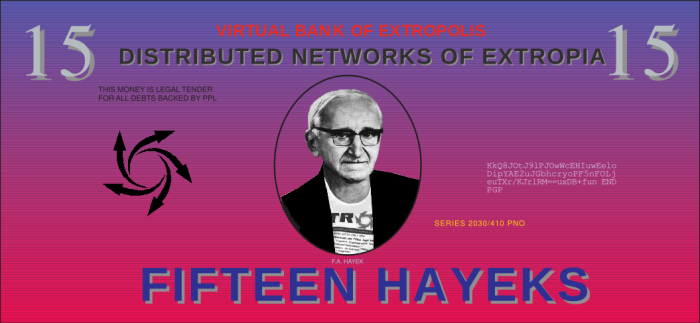
\includegraphics[scale=0.8]{img/fifteen-hayeks-note-extropy-15.png}
  \caption{Le billet fictif de 15 hayeks en couverture du magazine Extropy.}
\end{figure}

La monnaie numérique constituait donc l'un des sujets mis en avant par les extropiens. Mais ces derniers ne le faisaient pas autant que les cypherpunks qui, des années plus tard, tenteraient de mettre en pratique leur connaissance de la cryptographie pour en créer une.

\section*{Les cypherpunks}
\addcontentsline{toc}{section}{Les cypherpunks}

% Définition
Le mouvement cypherpunk est apparu en 1992 dans la Silicon Valley. Les cypherpunks étaient des gens qui prônaient l'utilisation proactive de la cryptographie en vue d'assurer la confidentialité et la liberté des individus dans le cyberespace. Ils s'opposaient à la surveillance, à la censure et à l'exploitation des données personnelles, et préconisaient la programmation et la publication ouverte de logiciels, préférablement sous licence libre, dans le but de les combattre.

% Terme cypherpunk
Le terme cypherpunk est un mot-valise composé des mots anglais \eng{cypher}, signifiant chiffre, dans le sens de code secret, et \eng{punk}, désignant originellement un voyou. Les cypherpunks étaient donc des rebelles amateurs de cryptographie. Le terme était directement calqué sur le mot cyberpunk, dont le préfixe cyber- fait référence à la cybernétique, la science des systèmes complexes et des réseaux, et pour cause~: le mouvement était partiellement issu du cyberpunk.

% Mouvement / genre cyberpunk
Le cyberpunk était un mouvement culturel construit autour de la littérature de science-fiction, qui s'inspirait à la fois de la sous-culture des punks et de la mouvance des hackers. Même si l'esthétique datait de la fin des années 70, le genre littéraire a largement été inauguré par l'écrivain William Gibson via la publication de ses premières nouvelles à partir de 1981 et surtout de son roman \emph{Neuromancien} en juillet 1984. Le mot a quant à lui a été inventé en 1983 par Bruce Bethke\sendnote{«~Comment ai-je créé ce mot~? De la même manière que n'importe quel nouveau mot, je suppose~: par la combinaison. J'ai pris une poignée de racines -- cyber, techno, etc. --, je les ai mélangées à un tas de termes désignant des jeunes socialement désorientés, et j'ai essayé les différentes combinaisons jusqu'à ce que l'une d'entre elles sonne tout simplement juste.~» -- Bruce Bethke, \eng{Cyberpunk: a short story by Bruce Bethke}, 1997~: \url{http://www.infinityplus.co.uk/stories/cpunk.htm}.} et popularisé par Gardner Dozois en décembre 1984 dans un éditorial pour le Washington Post\sendnote{Gardner Dozois, \eng{Science Fiction in the Eighties}, 30 décembre 1984~: \url{https://www.washingtonpost.com/archive/entertainment/books/1984/12/30/science-fiction-in-the-eighties/526c3a06-f123-4668-9127-33e33f57e313/}.}. % "How did I actually create the word? The way any new word comes into being, I guess: through synthesis. I took a handful of roots --cyber, techno, et al-- mixed them up with a bunch of terms for socially misdirected youth, and tried out the various combinations until one just plain sounded right."

% Combinaison de haute technologie et de bassesse humaine
La caractéristique principale du genre cyberpunk était de décrire un futur dystopique où la technique de pointe était omniprésente (implants informatiques, réalité augmentée, réalité virtuelle, intelligence artificielle, robots) et où la société était sujette à la consommation à outrance (drogue, sexe, etc.), au crime et à l'avarice de corporations. Le cyberpunk décrivait ainsi un monde combinant haute technologie et bassesse humaine, pour reprendre l'expression de Bruce Sterling\sendnote{Bruce Sterling, «~\eng{Preface}~», in \eng{Burning Chrome} (William Gibson), 1986.}, dont le héros tentait de s'extraire tant bien que mal. % "Gibson's classic one-two combination of lowlife and high-tech"

% Contreculture cyberdélique
De ce genre cyberpunk est né tout un mouvement d'individus qui partageaient la même vision du monde, formant notamment une contreculture cyberdélique, née de la fusion de cyberculture et du psychédélisme. Cette sous-culture en vogue dans la Silicon Valley était incarnée par la revue \eng{High Frontiers}, fondée en 1984 par R. U. Sirius, et qui est plus tard devenue \eng{Reality Hackers} puis \eng{Mondo 2000}.

% Différence avec les cypherpunks
Les cypherpunks étaient ainsi inspirés par ce mouvement. Toutefois, ils n'étaient pas pour autant des cyberpunks~: s'ils avaient bien conscience des scénarios dystopiques qui pouvaient dériver de l'évolution technique (notamment en ce qui concerne la surveillance), ils ne partageaient pas la même vision pessimiste relayée par le cyberpunk. De ce fait, le mouvement cypherpunk constituait en quelque sorte une réaction au cyberpunk, dans le sens où il postulait, à l'instar des extropiens, que l'évolution technique pouvait amener les êtres humains à s'émanciper plutôt qu'à tomber dans l'esclavage mutuel.

% True Names
Les cypherpunks basaient en particulier leurs réflexions sur une longue nouvelle publiée en 1980 par l'auteur de science-fiction Vernor Vinge, intitulée \eng{True Names}. Cette nouvelle, qui abordait des thèmes propres au genre cyberpunk sans en être strictement\sendnote{«~Je ne me considère certainement pas comme un écrivain cyberpunk. [...] Je pense que True Names partage un grand nombre d'idées techniques avec les récits cyberpunk. Je vois également deux différences substantielles entre True Names et les récits que l'on appelle généralement "cyberpunk". Premièrement, le cyberpunk montre davantage les aspects les plus sombres de la société future. Dans certains cas, il s'agit simplement d'un style dur à cuire. Dans d'autres cas, il capture la douleur d'un changement social très rapide. Deuxièmement, le cyberpunk est souvent pessimiste quant à la possibilité de changements sociaux et techniques, ce qui peut en fait être une très bonne chose.~» -- Vernor Vinge (interrogé par Michael Synergy), «~Hurtling Towards the Singularity~», \emph{Mondo 2000 issue 1}, 1989~: \url{https://archive.org/details/Mondo.2000.Issue.01.1989/page/n115/mode/2up}.}, contait l'histoire de Roger Pollack, un individu agissant au sein d'un groupe de pirates dans un monde virtuel appelé «~\eng{The Other Plane}~», qui utilisait le pseudonyme de Mr. Slippery et qui faisait attention à ne surtout pas révéler son «~Vrai Nom~» (à savoir son nom civil) au risque de subir une «~Vraie Mort~» (par exécution étatique). Cet enjeu correspondait ainsi à l'enjeu principal de la cryptographie~: la préservation de l'anonymat dans le but de conserver sa liberté et, \emph{in fine}, sa vie. % "I certainly don't think of myself as a cyberpunk writer. A couple of months ago, I was asked whether I thought True Names was cyberpunk. I wrote a note that appeared in Science Fiction Lovers. Let me just read that to you: "I think there's a large set of tech ideas that True Names shares with cyberpunk stories. I also see two substantial differences between True Names and the stories that are usually called 'cyberpunk.' One: cyberpunk shows more of future society's ugly underbelly. In some cases this is simply hardboiled style. In some cases, it captures the pain of very fast social change. Two: cyberpunk is often pessimistic about the possibility of social and technological change, which may in fact be a wonderfully good thing."

% Différence avec les extropiens
Les cypherpunks avaient ainsi le regard tourné vers l'avenir. Mais leur préoccupation concernaient surtout l'avenir proche~: c'était la confidentialité dans le cyberespace naissant\sendnote{Le terme «~cyberespace~» (\eng{cyberspace} en anglais) a été forgé par William Gibson dans sa nouvelle \emph{Gravé sur Chrome} publiée en juillet 1982, pour désigner la représentation virtuelle des flux de données sur Internet. Le terme «~matrice~» (\eng{matrix}) était utilisé en tant que synonyme.}. C'est pourquoi leur mouvement pouvait rassembler des optimistes et des pessimistes, des extropiens et des cyberpunks, qui trouvaient du sens dans cette lutte contre la surveillance de masse.

% Tim May
Le mouvement cypherpunk est initialement le fruit de la pensée et de l'action de Timothy C. May, dit «~Tim May~». Tim May était un scientifique, ingénieur et informaticien né en 1951 en périphérie de Washington D.C. Passionné de science-fiction et de physique, il avait travaillé pour Inter de 1974 où il avait contribué à résoudre le problème des particules alpha dans les circuits intégrés\sendnote{Timothy C. May, Murray H. Woods, \eng{Alpha-Particle-Induced Soft Errors in Dynamic Memories}, janvier 1979~: \url{https://gwern.net/doc/cs/hardware/1979-may.pdf}.}. Il avait accumulé une certaine fortune au cours de ces années, si bien qu'en 1986 (à l'âge de 35 ans), il décidait de prendre sa retraite pour se consacrer à ses passions politiques.

% Origine de l'idée cryptoanarchiste
Tim May a rencontré Phil Salin en 1987, par l'intermédiaire de Chip Morningstar\sendnote{Paralelní Polis, \eng{Timothy C. May - Thirty Years of Crypto Anarchy}, 11 février 2017~: \url{https://www.youtube.com/watch?v=TdmpAy1hI8g\&t=360s}.}. Il a ainsi pu discuter des implications de la cryptographie, avec Salin et sa femme, ainsi que d'autres personnes comme Marc Stiegler. C'est ce qui l'a poussé à écrire le \emph{Manifeste crypto anarchiste} en août 1988 qu'il a partagé avec Phil Salin et d'autres\sendnote{Timothy C. May, \eng{Cyphernomicon}, 16.3.4.}.

% Manifeste crypto anarchiste
Dans ce manifeste, il posait les bases de ce qui allait devenir la doctrine des cypherpunks et décrivait le potentiel d'émancipation individuelle apporté par la cryptographie et par l'anonymat. Le manifeste, pastiche ironique du \emph{Manifeste du parti communiste}, décrivait comment l'avènement des méthodes cryptographiques modernes allait, d'après lui, déstabiliser l'État en permettant aux individus d'échanger librement de l'information et de la richesse. En particulier, il écrivait~:

\begin{quote}
«~Tout comme la technique de l'imprimerie a altéré et réduit le pouvoir des corporations médiévales et la structure sociale de pouvoir, les méthodes cryptologiques altèrent fondamentalement la nature de l'interférence de l'État et des grandes entreprises dans les transactions économiques.\sendnote{Timothy C. May, \eng{The Crypto Anarchist Manifesto}, \wtime{22/11/1992 20:11:24 UTC}~: \url{https://cypherpunks.venona.com/date/1992/11/msg00204.html}.}~»
\end{quote} % "Just as the technology of printing altered and reduced the power of medieval guilds and the social power structure, so too will cryptologic methods fundamentally alter the nature of corporations and of government interference in economic transactions."

% Eric Hughes
Mais Tim May n'était pas seul à penser de cette manière et communiquait avec d'autres personnes qui partageaient ses idées. C'était le cas de son ami Eric Hughes, un jeune mathématicien et programmeur qui avait grandi dans une famille mormone en Virginie près de Washington et à Salt Lake City. Ce dernier avait travaillé brièvement pour DigiCash à Amsterdam avant de revenir sur la côte Ouest\sendnote{Timothy C. May, \eng{Hackers Conference Report}, \wtime{11/11/1992 08:55:26 UTC}~: \url{https://cypherpunks.venona.com/date/1992/11/msg00019.html}.}. En mai 1992, alors qu'il cherchait à emménager dans la Silicon Valley, lui et Tim May avaient longuement discuté de cryptographie, à tel point qu'ils ont décidé de reproduire ce type d'échange avec un plus grand nombre de personnes en organisant des réunions physiques. % Mormonisme d'Eric Hughes : cf. Crypto (Steven Levy), p. 259

% Première réunion
La première réunion du mouvement cypherpunk a eu lieu au cours de la journée du 19 septembre 1992, dans la maison d'Eric Hughes à Oakland. L'accès à cette réunion se faisait uniquement sur invitation afin de préserver la discrétion du mouvement. Libertariens pour la plupart, extropiens pour certains, les invités étaient des connaissances de May et Hughes issues de la communauté des hackers et des entreprises informatiques de la région. Durant la réunion, Tim May y a lu le \emph{Manifeste crypto anarchiste}. Une animation sous la forme d'un «~jeu de la crypto anarchie~» a eu lieu~: ce jeu consistait à simuler un réseau de mélange par l'échange et l'ouverture d'enveloppes de papier.\sendnote{Certains détails de la formation des cypherpunks sont issus de l'ouvrage \eng{Crypto: How the Code Rebels Beat the Government--Saving Privacy in the Digital Age} (pp. 257 -- 266) de Steven Levy publié en 2001.}

% John Gilmore, né en 1955
Parmi les invités se trouvait John Gilmore, un informaticien américain qui avait été l'un des premiers employés de Sun Microsystems. Il avait co-créé la hiérarchie ouverte alt.* sur Usenet et il était un contributeur majeur du projet GNU. Alors en retraite anticipé depuis 1986, tout comme May, il s'était engagé dans l'activisme dans le but de protéger les libertés civiles sur Internet. En 1989, il était le co-fondateur de Cygnus Support, une entreprise spécialisée dans le support professionnel de composants fondés sur GNU. Il a également co-fondé l'\eng{Electronic Frontier Foundation} (EFF) en 1990 aux côtés de Mitch Kapor et de John Perry Barlow, qui était une ONG internationale de protection des libertés sur Internet. Lui aussi voyait la cryptographie comme une moyen de libération individuelle\sendnote{«~Et si nous pouvions construire une société dans laquelle les informations ne seraient jamais collectées~? [...] C'est le genre de société que je veux construire.  Je veux que soit garantie - par la physique et la mathématique, pas par des lois - la possibilité de bénéficier de choses telles qu'une véritable confidentialité des communications personnelles, [...] une véritable confidentialité des enregistrements personnels, [...] une véritable liberté de commerce, [...] une véritable confidentialité financière [et] une véritable contrôle de l'identification.~» -- John Gilmore, \eng{Privacy, Technology, and the Open Society}, 28 mars 1991~: \url{http://www.toad.com/gnu/cfp.talk.txt}~; archive~: \url{https://web.archive.org/web/19991003163945/http://www.toad.com/gnu/cfp.talk.txt}.}. % "What if we could build a society where the information was never collected?  Where you could pay to rent a video without leaving a credit card number or a bank number?  Where you could prove you're certified to drive without ever giving your name?  Where you could send and receive messages without revealing your physical location, like an electronic post office box? That's the kind of society I want to build.  I want a guarantee -- with physics and mathematics, not with laws -- that we can give ourselves things like real privacy of personal communications, (...) real privacy of personal records, (...) real freedom of trade, (...) real financial privacy, (...) real control of identification." %

% Judith Milhon
Une autre personne présente durant cette réunion fondatrice était l'activiste Judith Milhon, une femme née en 1939 qui avait participé au mouvement des droits civiques pour l'abolition des discriminations raciales dans les années 60 et avait été emprisonnée pour désobéissance civile\sendnote{Sean Dodson, \eng{Judith Milhon: making the Internet a feminist issue}, 8 août 2003~: \url{https://www.theguardian.com/technology/2003/aug/08/guardianobituaries.obituaries}.}. Programmeuse, hackeuse, elle était alors la co-éditrice de la revue cyberpunk \eng{Mondo 2000}, à laquelle elle participait sous le nom de plume de St. Jude. Elle était également la compagne d'Eric Hughes, malgré leur grande différence d'âge.

% Terme cypherpunk
C'est elle qui a donné leur nom aux cypherpunks lors de cette réunion, sur le ton de la plaisanterie. «~Je pense que vous êtes des cryptoanarchistes -- ce que j'appellerais des cypherpunks~!~», a-t-elle écrit par la suite\sendnote{Judith Milhon, \eng{secretions}, \wtime{25/09/1992 10:01:26 UTC}~: \url{https://cypherpunks.venona.com/date/1992/09/msg00013.html}.}. Le terme capturait bien l'esprit de la cryptoanarchie, tout en donnant au mouvement un côté moins formel et dogmatique. En particulier, les gens préoccupés par ces enjeux n'étaient pas tous anarchistes~: ils pouvaient s'opposer fermement à l'autoritarisme et à la surveillance, sans pour autant vouloir remettre en cause les fondements même de l'État\sendnote{«~De plus, cela donne à tort l'impression que "cypherpunk" est synonyme d'"anarchiste". Il se trouve que je suis anarchiste, mais ce n'est pas ce en quoi croient la plupart des personnes associées au terme "cypherpunk", et il n'est pas juste de les dépeindre ainsi - bon sang, de nombreuses personnes sur cette liste de diffusion sont ouvertement hostiles à l'anarchisme. Je ne veux pas que les gens pensent qu'il faut détester l'idée même d'État pour aimer la cryptographie.~» -- Perry E. Metzger, \eng{Re: PC Expo summary!!}, \wtime{01/07/1994 12:13:09 UTC}~: \url{https://cypherpunks.venona.com/date/1994/07/msg00014.html}.}. C'est ce côté indéfini et décontracté qui a fait que le terme a été adopté immédiatement. % "Also, it unfairly makes it look like "cypherpunk" means "anarchist". Now, it happpens that I am an anarchist, but that isn't what most people associated with the term "cypherpunk" believe in, and it isn't fair to paint them that way -- hell, many people on this mailing list are overtly hostile to anarchism. I don't want people to think you have to hate the idea of government in order to like cryptography."

% Création de la mailing list
Après la réunion, Eric Hughes, avec l'aide de Hugh Daniel, a créé une liste de diffusion de courrier électronique nommée «~Cypherpunks~». Le courriel de bienvenue\sendnote{Eric Hughes, \eng{No Subject}, \wtime{22 Sep 92 05:43:46 UTC}~: \url{https://cypherpunks.venona.com/date/1992/09/msg00001.html}.} a été envoyé dans la soirée du 21 septembre (PDT). La liste était relayée par le serveur associé au nom de domaine \texttt{toad.com} appartenant à John Gilmore. Ce dernier a aussi offert la disponibilité des locaux de Cygnus pour les réunions ultérieures.

% Succès de la liste
La liste a accueilli de nombreuses discussions relatives à la cryptographie et à son utilisation concrète, dont notamment l'argent liquide électronique. Beaucoup de gens sont intervenus dès les premiers mois, comme par exemple l'ancien pirate téléphonique John Draper. En un an à peine, la liste recensait ainsi plus de 500 participants. % Source : Cyphernomicon 3.3.14

% Hal Finney
L'un de ces participants était Harold T. Finney \textsc{ii}, dit «~Hal Finney~», informaticien et cryptographe américain, diplômé de Caltech et programmeur de jeux vidéos pour les consoles Intellivision et Atari VCS. Extropien et enthousiasmé la popularisation d'Internet, il était obsédé par la cryptographie, à tel point qu'il était rentré en contact avec Phil Zimmermann pour travailler avec lui sur la version 2.0 de PGP, qui était sortie le 2 septembre 1992. Hal Finney était aussi fasciné par les idées de David Chaum. En novembre 1992, il écrivait à la liste de diffusion~:

\begin{quote}
«~Nous voici confrontés aux problèmes de la perte de confidentialité, de l'informatique trompeuse, des bases de données massives, de l'augmentation de la centralisation -- et Chaum propose une direction à suivre complètement différente, une direction qui met le pouvoir entre les mains des individus plutôt que celles des États et des grandes entreprises. L'ordinateur peut être utilisé comme un outil pour libérer et protéger les personnes, plutôt que pour les contrôler.\sendnote{Hal Finney, \eng{Why remailers...}, \wtime{16/11/1992 01:30:02 UTC}~: \url{https://cypherpunks.venona.com/date/1992/11/msg00108.html}.}~»
\end{quote}

% Appel à la pratique
La vision des cypherpunks était claire~: mettre en pratique ce qui avait été jusque-là de vagues spéculations. Il était en effet stérile de théoriser des choses si cela ne se traduisait pas par des actions concrètes. Cet esprit pratique a été parfaitement résumé par Eric Hughes dans son \emph{Manifeste d'un Cypherpunk} envoyé à la liste de diffusion en mars 1993, où il écrivait alors~:

\begin{quote}
«~Nous devons défendre notre propre vie privée si nous voulons en avoir une. Nous devons nous rassembler et créer des systèmes qui rendent possibles les transactions anonymes. Depuis des siècles, les gens défendent leur vie privée par des chuchotements, par l'obscurité, par des enveloppes, des portes fermées, des poignées de main secrètes et des messagers. Les techniques du passé ne permettaient pas une forte confidentialité, mais les techniques électroniques le permettent.

Nous, les Cypherpunks, nous consacrons à construire des systèmes anonymes. Nous défendons notre confidentialité avec la cryptographie, avec les systèmes anonymes de transfert de courriels, avec les signatures numériques, et avec la monnaie électronique.

Les Cypherpunks écrivent du code. Nous savons que quelqu'un doit écrire un logiciel pour défendre la vie privée, et puisque nous ne pouvons pas avoir de vie privée si nous ne le faisons pas tous, nous allons l'écrire. Nous publions notre code pour que nos collègues Cypherpunks puissent le mettre en pratique et expérimenter avec. Notre code est libre d'utilisation pour tous, dans le monde entier. Nous ne nous soucions guère que vous n'approuviez pas les logiciels que nous écrivons. Nous savons que les logiciels ne peuvent pas être détruits et qu'un système largement dispersé ne peut pas être arrêté.\sendnote{Eric Hughes, \eng{RANTS: A Cypherpunk's Manifesto}, \wtime{17/03/1993 19:51:06 UTC}~: \url{https://cypherpunks.venona.com/date/1993/03/msg00392.html}.}~»
\end{quote} % "We must defend our own privacy if we expect to have any.  We must come together and create systems which allow anonymous transactions to take place.  People have been defending their own privacy for centuries with whispers, darkness, envelopes, closed doors, secret handshakes, and couriers.  The technologies of the past did not allow for strong privacy, but electronic technologies do.
%
% We the Cypherpunks are dedicated to building anonymous systems.  We are defending our privacy with cryptography, with anonymous mail forwarding systems, with digital signatures, and with electronic money.
%
% Cypherpunks write code.  We know that someone has to write software to defend privacy, and since we can't get privacy unless we all do, we're going to write it. We publish our code so that our fellow Cypherpunks may practice and play with it. Our code is free for all to use, worldwide.  We don't much care if you don't approve of the software we write.  We know that software can't be destroyed and that a widely dispersed system can't be shut down."

% Publicité
Deux mois plus tard, en mai 93, le mouvement était définitivement lancé~: les cypherpunks faisaient la une du magazine Wired, récemment fondé dans le but de parler de l'incidence culturelle, économique et politique des techniques émergentes. Tim May, Eric Hughes et John Gilmore apparaissaient masqués sur la couverture, et un long article détaillait leurs idées et leurs revendications\sendnote{Steven Levy, \eng{Crypto Rebels}, 1\ier{} février 1993~: \url{https://www.wired.com/1993/02/crypto-rebels/}~; archive~: \url{https://web.archive.org/web/20151102012232/https://www.wired.com/1993/02/crypto-rebels/}.}. Les cypherpunks ont également été présentés par la suite dans les revues \eng{Whole Earth Review} et \eng{The Village Voice}\sendnote{\eng{Cypherpunks, e-Money and the Technologies of Disconnection}~: \url{https://archive.org/details/sim_whole-earth_summer-1993_79/page/40/mode/2up}~; \url{http://www.juliandibbell.com/texts/codewars.html}.}.

\section*{Les accomplissements des cypherpunks}
\addcontentsline{toc}{section}{Les accomplissements des cypherpunks}

Le mouvement cypherpunk est né juste après le triomphe des États-Unis dans la guerre froide les opposant à l'URSS et au début de la démocratisation d'Internet, amorcée notamment par la popularisation de Usenet et par l'apparition du World Wide Web. Il est apparu en quelque sorte au bon moment pour alerter et accompagner ce qui allait suivre.

% --- Guerre contre la cryptographie ---

\textbf{Guerre contre la cryptographie.} Le premier accomplissement des cypherpunks a été leur rôle dans la guerre contre la cryptographie, orchestrée par l'État fédéral étasunien.

La première réaction étatique a été la guerre contre PGP. La version 1.0 de PGP avait été publiée sur Internet en juin 1991 et la version 2.0 en septembre 1992, en dehors des États-Unis. En 1993, le logiciel de chiffrement commençait à se populariser.

Lorsque Phil Zimmermann a publié la version 1.0 de PGP par le biais de \eng{bulletin board systems} et de Usenet en juin 1991, il savait qu'il risquait d'attiser une réponse du pouvoir. La Réglementation américaine sur le trafic d'armes au niveau international (\eng{International Traffic in Arms Regulations} en anglais ou ITAR) considérait en effet les produits cryptographiques comme des «~munitions~» et en interdisait l'exportation sans licence. Par conséquent, une enquête contre Zimmermann a été ouverte par l'État fédéral en février 1993.

% Réaction
Cette décision a naturellement provoqué une forte résistance de la part des cypherpunks qui, en réponse à cette loi absurde, se sont mis à partager le code de chiffrement dans une démarche de désobéissance civile. Le jeune britannique Adam Back l'a fait imprimer sur des t-shirts qu'il distribuait aux autres et certains ont été jusqu'à se le tatouer sur leur corps\sendnote{\url{http://www.cypherspace.org/adam/rsa/}}. En 1995, Phil Zimmermann a publié la version 2.6.2 de PGP dans un livre\sendnote{Philip Zimmermann, \eng{PGP: Source Code and Internals}, 1995~: \url{https://philzimmermann.com/EN/essays/BookPreface.html}.}, dans le but de réduire au maximum la distinction entre le code et l'expression, cette dernière étant protégée par le premier amendement de la Constitution des États-Unis. Il a bénéficié au passage du soutien du MIT\sendnote{Steven Levy, \eng{Cypher Wars}, 1994~: \url{https://www.wired.com/1994/11/cypher-wars/}~; archive~: \url{https://web.archive.org/web/20160403024823/https://www.wired.com/1994/11/cypher-wars/}.}.

Les charges contre Zimmermann ont finalement été abandonnées en 1996, lui permettant de créer son entreprise pour travailler sur PGP et d'engager des employés, comme Hal Finney. En novembre de la même année, Bill Clinton signait l'Ordre exécutif 13026 qui assouplissait considérablement les restrictions sur l'exportation des produits cryptographiques.

\textbf{Clipper.} Cependant, la guerre contre la cryptographie ne s'arrêtait pas là. Elle ne concernait en effet pas que les interdictions, mais aussi les obligations. Le projet de loi sénatoriale 266, proposé par Joe Biden en 1991, devait ainsi imposer l'existence d'une porte dérobée dans tous les appareils de communication~: % Joe Biden's S.266

\begin{quote}
«~Le Congrès estime que les fournisseurs de services de communications électroniques et les fabricants d'équipements de services de communications électroniques doivent veiller à ce que les systèmes de communications permettent au gouvernement d'obtenir le contenu en texte clair des communications vocales, de données et autres lorsque la loi l'autorise de manière appropriée.\sendnote{\eng{Comprehensive Counter-Terrorism Act of 1991}, 24 janvier 1991~: \url{https://www.congress.gov/bill/102nd-congress/senate-bill/266/text}.}~»
\end{quote} % "It is the sense of Congress that providers of electronic communications services and manufacturers of electronic communications service equipment shall ensure that communications systems permit the government to obtain the plain text contents of voice, data, and other communications when appropriately authorized by law."

% Puce Clipper
Ce projet s'est matérialisé le 16 avril 1993 par l'annonce par la Maison-Blanche de la puce Clipper, un cryptoprocesseur servant à chiffrer les messages vocaux et les données, qui implémentait (au travers de son algorithme Skipjack) un dispositif d'autorité de séquestre permettant aux agences étasuniennes de déchiffrer les communications au besoin. Cette puce était développée et produite par la NSA et était destinée à équiper les appareils électroniques vendus au grand public. La Maison-Blanche se justifiait en prétendant que la puce pourrait «~à la fois fournir aux citoyens respectueux de la loi un accès au chiffrement dont ils ont besoin et empêcher les criminels de l'utiliser pour cacher leurs activités illégales\sendnote{The White House, \eng{White House Annoucement of the Clipper Initiative}, 16 avril 1993~: \url{https://groups.csail.mit.edu/mac/classes/6.805/articles/crypto/clipper-announcement.html}.}~».

% Lutte contre Clipper
Cette annonce n'a pas manqué de faire réagir les cypherpunks qui se sont opposés en bloc à ce projet orwellien. Cependant, la lutte n'a pas été longue~: en juin 1994, le cypherpunk Matt Blaze a découvert une vulnérabilité au sein du dispositif d'autorité de séquestre\sendnote{John Markoff, \eng{At AT\&T, No Joy on Clipper Flaw}, 3 juin 1994~: \url{https://www.nytimes.com/1994/06/03/business/at-at-t-no-joy-on-clipper-flaw.html}~; Matt Blaze, \eng{Paper available via ftp}, \wtime{05/06/1994 00:01:57 UTC}~: \url{https://cypherpunks.venona.com/date/1994/06/msg00319.html}.}, qui rendait le dispositif inefficace et permettait à la puce d'être utilisée pour chiffrer les données normalement. À partir de là, le projet a perdu progressivement en ampleur pour être définitivement abandonné en 1996\sendnote{Cette victoire n'a cependant pas empêché pas les agences étasuniennes d'espionner leur propre population de manière massive, comme l'ont montré les révélations d'Edward Snowden en 2013. -- Voir Glenn Greenwald, \eng{NSA collecting phone records of millions of Verizon customers daily}, 6 juin 2013~: \url{https://www.theguardian.com/world/2013/jun/06/nsa-phone-records-verizon-court-order}.}. Le cyberespace était déclaré indépendant\sendnote{John Perry Barlow, \eng{A Declaration of the Independence of Cyberspace}, 8 février 1996~: \url{https://www.eff.org/fr/cyberspace-independence}.}.

% --- Autres accomplissements ---

Comme on l'a observé, l'optique des cypherpunks était d'être dans l'action, d'écrire du code et de partager du code qui puisse être utilisé. Ils se sont donc focalisés sur la construction de systèmes axés sur trois aspects majeurs~: la protection de la vie privée, la diffusion de l'information et le commerce en ligne. % combinaison de techniques cryptographiques permettant d'assurer la confidentialité, l'authenticité et l'intégrité des données. Réputation.

% Serveurs de courriel anonymes (remailers)
Le premier domaine d'innovation a été celui des serveurs de courriel anonyme, qui permettaient de retransmettre les courriers électroniques de façon à masquer l'identité de leur expéditeur. Le premier serveur de ce type a mis en place par Eric Hughes et Hal Finney pour la liste des cypherpunks dès octobre 1992, il utilisait PGP pour le chiffrement\sendnote{Hal Finney, \eng{New remailer...}, \wtime{13/10/1992 20:31:48 UTC}~: \url{https://cypherpunks.venona.com/date/1992/10/msg00082.html}.}. En 1994, Lance Cottrell a amélioré la chose en proposant Mixmaster\sendnote{Lance Cottrell, \eng{1st Draft Mixmaster chaining instructions}, \wtime{21/11/1994 01:07:02 UTC}~: \url{https://cypherpunks.venona.com/date/1994/11/msg00158.html}.}, qui permettait d'envoyer des courriels par paquets de taille fixe et de les réordonner, pour empêcher le traçage des courriels par la surveillance de l'activité du serveur. % Cypherpunks remailer: type I (1992); Mixmaster remailer: type II (1994); Mixminion remailer: type III (2002)

% Navigation
Outre le courriel, l'objectif des cypherpunks était de rendre la navigation sur Internet plus anonyme. L'émergence du Web était jugée trop transparente.

% Réseau Freedom
C'était l'idée des frères Austin et Hamnett Hill qui ont lancé le réseau Freedom en 1999 par l'intermédiaire de leur entreprise Zero-Knowledge Systems, qui employait notamment les cypherpunks Ian Goldberg et Adam Back\sendnote{Chris Oakes, \eng{Zero-Knowledge: Nothing Personal}, 9 février 1999~: \url{https://www.wired.com/1999/02/zero-knowledge-nothing-personal/}.}. Mais cette expérience s'est arrêtée en 2001, faute d'utilisation suffisante.

% Tor
Un autre projet dans lequel les cypherpunks se sont impliqués est le réseau Tor, qui fonctionne comme on l'a déjà expliqué grâce au routage en ognon, d'où son nom (Tor est l'acronyme de \eng{The Onion Router}. En effet, si Tor est le résultat d'une recherche militaire provenant de la Navy, les individus qui ont travaillé sur son implémentation n'en avaient pas moins des convictions allant dans le sens des cypherpunks. Roger Dingledine et Nick Mathewson, les deux informaticiens qui ont aidé Paul Syverson dans cette conceptions, en faisaient partie~: le premier était derrière le projet Free Haven, qui avait pour but de développer un système décentralisé de stockage de données\sendnote{\url{https://www.freehaven.net/}}~; le second est crédité pour avoir créé le programme de serveur de courriel anonyme Mixminion\sendnote{George Danezis, Roger Dingledine, Nick Mathewson, \eng{Mixminion: Design of a Type III Anonymous Remailer Protocol}, 2003~: \url{https://git.gnunet.org/bibliography.git/plain/docs/minion-design.pdf}.}. On peut également citer le jeune Jacob Appelbaum, qui s'est fortement impliqué dans le projet Tor entre 2004 et 2016.

% BlackNet
Un troisième accomplissement a été la fluidification des flux informationnels, notamment face à la censure. En 1993, Tim May a repris le modèle de l'AMIX de Phil Salin pour introduire un concept de place de marché de l'information appelé BlackNet. Cette plateforme devait servir à échanger des secrets commerciaux, des recettes de fabrication, des techniques relatives aux nanotechnologies, des informations sur les décisions d'entreprises, au moyen de «~CryptoCredits~», la monnaie interne du système. Il s'agissait donc de libérer l'information des contraintes étatiques~: «~BlackNet est officiellement non idéologique, mais considère les États-nations, les lois d'exportation, les lois sur les brevets, les considérations de sécurité nationale, etc. comme des reliques de l'ère pré-cyberspatiale~», écrivait Tim May\sendnote{Timothy C. May, \eng{no subject (file transmission)}, 17 août 1993, \url{https://cypherpunks.venona.com/date/1993/08/msg00538.html}.}.

% Autres, Cryptome
Le concept de BlackNet était une simple expérience de pensée et n'a jamais été mis en œuvre. Toutefois, il a préfiguré d'autres modèles qui ont ouvert la voie au partage d'informations sensibles sur Internet. C'était par exemple le cas de Cryptome, un site web lancé en 1996 par le cypherpunk John Young pour héberger des documents sensibles et censurés par les États\sendnote{\eng{Cryptome JYA Archive}~: \url{https://cryptome.org/jya/}.}.

% WikiLeaks
Mais c'était surtout le cas de WikiLeaks, la plateforme facilitant la publication de documents classifiés fondée en 2006 par l'informaticien australien Julian Assange. Julian Assange était un cypherpunk assumé~: il envoyait des courriels sur la liste depuis au moins 1995 et a par la suite co-écrit un livre à ce sujet\sendnote{Julian Assange, Jacob Appelbaum, Andy Müller-Maguhn, Jérémie Zimmermann, \eng{Cypherpunks: Freedom and the Future of the Internet}, 2012.}. WikiLeaks a permis le développement de l'activité des lanceurs d'alertes ou des \eng{whistleblowers} qui révèlent les agissements illégaux ou injustes de leurs employeurs, et en particulier des États, largement inaugurée par la publication des Pentagon Papers en 1971 par Daniel Ellsberg. Grâce à l'utilisation du chiffrement et de Tor, WikiLeaks permettait aux personnes à l'origine des fuites de conserver leur anonymat.

% Mojo Nation
Enfin, sur un autre plan, les cypherpunks se sont également investis dans le développement du pair-à-pair. En 2000, le développeur Jim McCoy, cypherpunk de la première heure, a ainsi lancé Mojo Nation, un projet de plateforme d'échange de fichiers en pair-à-pair intégrant une devise interne\sendnote{Damien Cave, \eng{The Mojo solution}, 9 octobre 2000~: \url{https://www.salon.com/2000/10/09/mojo_nation/}.}. En 2001, Bram Cohen, qui travaillait avec lui a quitté le projet et lancé BitTorrent, qui est devenu la référence pour le partage de fichiers au cours des années. Mojo Nation, alors renommé en Mnet, a été repris par Zooko Wilcox, qui a lancé son propre système en 2006 sous le nom de Tahoe-LAFS (et qui a ensuite contribué à lancer ZCash en 2016). % TAZ "temporary autonomous zone" Hakim Bey, 1991

% Cybermonnaie
Mais ce qu'il manquait à tous ces systèmes, c'était une monnaie numérique robuste qui soit adaptée au cyberespace, chose à laquelle les cypherpunks aspiraient depuis le début. Leurs modèles possédaient parfois des unités de compte internes, mais elles étaient très instables. Malheureusement, une telle monnaie ne serait conçue que des années plus tard, en 2008, au travers de Bitcoin.

% Silk Road : BlackNet précédait aussi aussi en quelque sorte la place de marché Silk Road, créée par Ross Ulbricht en 2011, qui a été essentiellement utilisée pour la vente de drogues diverses.
% Le tristement célèbre concept d'Assassination Politics\sendnote{\url{https://cryptome.org/ap.htm}~; mentionné sur cypherpunks en déc. 1995~: \url{https://cypherpunks.venona.com/date/1995/12/msg00570.html}, \url{https://cypherpunks.venona.com/date/1995/12/msg00928.html}}.

\section*{Une guerre perpétuelle}
\addcontentsline{toc}{section}{Une guerre perpétuelle}

Bitcoin s'inscrit pleinement dans la guerre technologique opposant l'autorité à la liberté. Son code n'est pas neutre~: il n'est pas une vague technique qu'on puisse utiliser dans un sens ou dans l'autre, mais il a pour objectif clair d'amener plus de liberté individuelle.

Bitcoin est issu d'idéologies qui appellent à la pratique~: les libristes appelaient à la publication sous licence libre dans le but de mettre en commun l'ensemble des connaissances de l'humanité, les extropiens appelaient à la recherche et à l'expérimentation pour améliorer drastiquement les conditions de vie matérielles de l'être humain, les cypherpunks appelaient à écrire du code afin de préserver la confidentialité des individus dans le cyberespace.

Satoshi Nakamoto était-il un cypherpunk~? Sans en faire pleinement partie et sans s'en réclamer, le créateur de Bitcoin était clairement influencé par l'héritage cypherpunk. D'abord, il a utilisé un pseudonyme et, par de bonnes pratiques, comme l'utilisation de PGP, de Tor et de Namecheap, il est parvenu à préserver son anonymat malgré presque trois années d'activité en ligne. Puis, il a publié le livre blanc sur la liste de diffusion dédiée à la cryptographie gérée par Perry Metzger, qui était la digne héritière de la liste cypherpunk, qui avait malheureusement périclité à la fin des années 90. Ensuite, il semblait démontrer une bonne connaissance de ce qui s'était passé et de ce qui avait été fait avant lui, malgré quelques lacunes. Enfin, il a programmé un outil pour arriver à un résultat émancipateur. Il semble donc raisonnable d'assimiler Satoshi aux cypherpunks tout en gardant en tête qu'il a toujours été mesuré dans ses quelques jugements politiques.

% Clé PGP de Satoshi : \sendnote{\url{https://bitcointalk.org/index.php?topic=458.msg5772\#msg5772}}

\printendnotes

\backmatter

\printendnotes

{\footnotesize \printnotes}

\end{document}